% Options for packages loaded elsewhere
\PassOptionsToPackage{unicode}{hyperref}
\PassOptionsToPackage{hyphens}{url}
%
\documentclass[
]{book}
\usepackage{lmodern}
\usepackage{amssymb,amsmath}
\usepackage{ifxetex,ifluatex}
\ifnum 0\ifxetex 1\fi\ifluatex 1\fi=0 % if pdftex
  \usepackage[T1]{fontenc}
  \usepackage[utf8]{inputenc}
  \usepackage{textcomp} % provide euro and other symbols
\else % if luatex or xetex
  \usepackage{unicode-math}
  \defaultfontfeatures{Scale=MatchLowercase}
  \defaultfontfeatures[\rmfamily]{Ligatures=TeX,Scale=1}
\fi
% Use upquote if available, for straight quotes in verbatim environments
\IfFileExists{upquote.sty}{\usepackage{upquote}}{}
\IfFileExists{microtype.sty}{% use microtype if available
  \usepackage[]{microtype}
  \UseMicrotypeSet[protrusion]{basicmath} % disable protrusion for tt fonts
}{}
\makeatletter
\@ifundefined{KOMAClassName}{% if non-KOMA class
  \IfFileExists{parskip.sty}{%
    \usepackage{parskip}
  }{% else
    \setlength{\parindent}{0pt}
    \setlength{\parskip}{6pt plus 2pt minus 1pt}}
}{% if KOMA class
  \KOMAoptions{parskip=half}}
\makeatother
\usepackage{xcolor}
\IfFileExists{xurl.sty}{\usepackage{xurl}}{} % add URL line breaks if available
\IfFileExists{bookmark.sty}{\usepackage{bookmark}}{\usepackage{hyperref}}
\hypersetup{
  pdftitle={ESOC 2014 Introduction to Data Science},
  pdfauthor={Adriana Picoral, PhD (she/her)  adrianaps@email.arizona.edu   The University of Arizona sits on the homelands of the Tohono O'odham and Yaqui, whose care and keeping of these lands allows us to be here today.},
  hidelinks,
  pdfcreator={LaTeX via pandoc}}
\urlstyle{same} % disable monospaced font for URLs
\usepackage{color}
\usepackage{fancyvrb}
\newcommand{\VerbBar}{|}
\newcommand{\VERB}{\Verb[commandchars=\\\{\}]}
\DefineVerbatimEnvironment{Highlighting}{Verbatim}{commandchars=\\\{\}}
% Add ',fontsize=\small' for more characters per line
\usepackage{framed}
\definecolor{shadecolor}{RGB}{248,248,248}
\newenvironment{Shaded}{\begin{snugshade}}{\end{snugshade}}
\newcommand{\AlertTok}[1]{\textcolor[rgb]{0.94,0.16,0.16}{#1}}
\newcommand{\AnnotationTok}[1]{\textcolor[rgb]{0.56,0.35,0.01}{\textbf{\textit{#1}}}}
\newcommand{\AttributeTok}[1]{\textcolor[rgb]{0.77,0.63,0.00}{#1}}
\newcommand{\BaseNTok}[1]{\textcolor[rgb]{0.00,0.00,0.81}{#1}}
\newcommand{\BuiltInTok}[1]{#1}
\newcommand{\CharTok}[1]{\textcolor[rgb]{0.31,0.60,0.02}{#1}}
\newcommand{\CommentTok}[1]{\textcolor[rgb]{0.56,0.35,0.01}{\textit{#1}}}
\newcommand{\CommentVarTok}[1]{\textcolor[rgb]{0.56,0.35,0.01}{\textbf{\textit{#1}}}}
\newcommand{\ConstantTok}[1]{\textcolor[rgb]{0.00,0.00,0.00}{#1}}
\newcommand{\ControlFlowTok}[1]{\textcolor[rgb]{0.13,0.29,0.53}{\textbf{#1}}}
\newcommand{\DataTypeTok}[1]{\textcolor[rgb]{0.13,0.29,0.53}{#1}}
\newcommand{\DecValTok}[1]{\textcolor[rgb]{0.00,0.00,0.81}{#1}}
\newcommand{\DocumentationTok}[1]{\textcolor[rgb]{0.56,0.35,0.01}{\textbf{\textit{#1}}}}
\newcommand{\ErrorTok}[1]{\textcolor[rgb]{0.64,0.00,0.00}{\textbf{#1}}}
\newcommand{\ExtensionTok}[1]{#1}
\newcommand{\FloatTok}[1]{\textcolor[rgb]{0.00,0.00,0.81}{#1}}
\newcommand{\FunctionTok}[1]{\textcolor[rgb]{0.00,0.00,0.00}{#1}}
\newcommand{\ImportTok}[1]{#1}
\newcommand{\InformationTok}[1]{\textcolor[rgb]{0.56,0.35,0.01}{\textbf{\textit{#1}}}}
\newcommand{\KeywordTok}[1]{\textcolor[rgb]{0.13,0.29,0.53}{\textbf{#1}}}
\newcommand{\NormalTok}[1]{#1}
\newcommand{\OperatorTok}[1]{\textcolor[rgb]{0.81,0.36,0.00}{\textbf{#1}}}
\newcommand{\OtherTok}[1]{\textcolor[rgb]{0.56,0.35,0.01}{#1}}
\newcommand{\PreprocessorTok}[1]{\textcolor[rgb]{0.56,0.35,0.01}{\textit{#1}}}
\newcommand{\RegionMarkerTok}[1]{#1}
\newcommand{\SpecialCharTok}[1]{\textcolor[rgb]{0.00,0.00,0.00}{#1}}
\newcommand{\SpecialStringTok}[1]{\textcolor[rgb]{0.31,0.60,0.02}{#1}}
\newcommand{\StringTok}[1]{\textcolor[rgb]{0.31,0.60,0.02}{#1}}
\newcommand{\VariableTok}[1]{\textcolor[rgb]{0.00,0.00,0.00}{#1}}
\newcommand{\VerbatimStringTok}[1]{\textcolor[rgb]{0.31,0.60,0.02}{#1}}
\newcommand{\WarningTok}[1]{\textcolor[rgb]{0.56,0.35,0.01}{\textbf{\textit{#1}}}}
\usepackage{longtable,booktabs}
% Correct order of tables after \paragraph or \subparagraph
\usepackage{etoolbox}
\makeatletter
\patchcmd\longtable{\par}{\if@noskipsec\mbox{}\fi\par}{}{}
\makeatother
% Allow footnotes in longtable head/foot
\IfFileExists{footnotehyper.sty}{\usepackage{footnotehyper}}{\usepackage{footnote}}
\makesavenoteenv{longtable}
\usepackage{graphicx,grffile}
\makeatletter
\def\maxwidth{\ifdim\Gin@nat@width>\linewidth\linewidth\else\Gin@nat@width\fi}
\def\maxheight{\ifdim\Gin@nat@height>\textheight\textheight\else\Gin@nat@height\fi}
\makeatother
% Scale images if necessary, so that they will not overflow the page
% margins by default, and it is still possible to overwrite the defaults
% using explicit options in \includegraphics[width, height, ...]{}
\setkeys{Gin}{width=\maxwidth,height=\maxheight,keepaspectratio}
% Set default figure placement to htbp
\makeatletter
\def\fps@figure{htbp}
\makeatother
\setlength{\emergencystretch}{3em} % prevent overfull lines
\providecommand{\tightlist}{%
  \setlength{\itemsep}{0pt}\setlength{\parskip}{0pt}}
\setcounter{secnumdepth}{5}
\usepackage{booktabs}
\usepackage[]{natbib}
\bibliographystyle{apalike}

\title{ESOC 2014 Introduction to Data Science}
\author{Adriana Picoral, PhD (she/her) \href{mailto:adrianaps@email.arizona.edu}{\nolinkurl{adrianaps@email.arizona.edu}} The University of Arizona sits on the homelands of the Tohono O'odham and Yaqui, whose care and keeping of these lands allows us to be here today.}
\date{2020-08-14}

\begin{document}
\maketitle

{
\setcounter{tocdepth}{1}
\tableofcontents
}
\hypertarget{syllabus}{%
\chapter{Syllabus}\label{syllabus}}

\leavevmode\hypertarget{more_info}{}%
Tuesday \& Thursday 12:30pm - 1:45pm

\begin{itemize}
\tightlist
\item
  Final Exam Date: December 16 (Wednesday) 1:00pm - 3:00pm
\end{itemize}

Tuesday \& Thursday 2:00pm - 3:15pm

\begin{itemize}
\tightlist
\item
  Final Exam Date: December 14 (Monday) 3:30pm - 5:30pm
\end{itemize}

\textbf{Office Hours/Free help session/Work time}

\begin{itemize}
\tightlist
\item
  Tuesday 9:30am - 11:00am \& Wednesday 1:00pm - 2:30pm
\end{itemize}

\hypertarget{course-description}{%
\section{Course Description}\label{course-description}}

This course provides an introduction to the various skills and considerations required for data management and analysis in business, education, and science. Particular attention will be given to learning how to use the free and open-source computing environment R, as well as one of its data visualization packages, ggplot2.

\textbf{Upon completion of this course, students should be able to:}

\begin{enumerate}
\def\labelenumi{\arabic{enumi}.}
\item
  Understand data science as a process
\item
  Think critically about how data are stored, used, managed, analyzed, and presented
\item
  Engage in computational thinking and modeling
\item
  Experiment with skills required for large-scale data analysis
\end{enumerate}

This course is designed to be interactive and hands-on.

\hypertarget{a-few-words-on-r-and-coding}{%
\section{A Few Words on R and Coding}\label{a-few-words-on-r-and-coding}}

This course will be based around the programming language R which we will use within the integrated development environment (IDE) R Studio. For many of you this will be the first time programming, \textbf{AND THAT'S OK! This course is intended for beginners, and we will actively focus on building up your R skills over the course of the semester}. Of course, there will still be challenges along the way, but you will rapidly figure out how to solve your own problems as well as to apply your current knowledge to new and exciting questions. If you are struggling I highly encourage you to take advantage of my free help sessions (see times above). Of course, Google is always a super helpful way to get insight into coding problems. Our class Slack channel will also be there so you can help each other out. You might want to watch \href{https://www.youtube.com/watch?v=ZFaWxxzouCY}{Roger Peng's video on how to get help}, which contains guidelines on what information to provide when asking a question in a public forum.

I also want to note that I highly encourage you to help each other, as data scientists are rarely working in isolation. \textbf{This does not mean you can directly share code associated with an assignment (this is a violation of UA's Code of Academic Integrity)}. What it does mean is that it is helpful to talk to each other about problems you encountered, resources you found, or provide helpful tips.

Learning to code nowadays is much easier, since a simple Google search will research in a huge amount of code that can solve any number of problems. You may use online resources (e.g., StackOverflow), but we will go over the syntax needed to solve all assignments in class. If you do use any external resources, you must explicitly cite where the code was obtained in your comments (add a direct link to the resource). I'll be checking for recycled code, and any code you re-used without a proper citation will be treated as plagiarism.

\hypertarget{a-few-words-on-technology}{%
\section{A Few Words on Technology}\label{a-few-words-on-technology}}

\begin{enumerate}
\def\labelenumi{\arabic{enumi}.}
\item
  YOU MUST HAVE ACCESS TO A COMPUTER YOU CAN CODE WITH IN EVERY CLASS! We will be actively coding in R on a daily basis, and not being able to follow along will severely hamper your learning. If you do not have a laptop or yours had troubles at some point during the semester, the library offers fast and free rentals of both macs and PCs: \url{https://new.library.arizona.edu/tech/borrow}. You can also take advantage of the multiple computer labs on campus: \url{https://it.arizona.edu/service/oscr-computer-labs}
\item
  You will have access to and will be required to retrieve all course materials from the course page on GitHub.
\item
  You will need to have R and R Studio installed and functioning by the second day of class. We will go over what these programs are and how to install them in the first week of class.
\item
  Slack participation is critical! If you are having a coding issue, first try and solve it on your own. If you're still struggling, then post it to our Slack. Essentially, if you are about to email me with a homework/class/coding question, post it to Slack first. I'm not doing this to save me time, but rather because virtually all programmers/coders solve problems by helping each other, and thus I want you to do the same! Please \href{https://join.slack.com/t/ischool-esoc214/shared_invite/zt-gbmjw9oz-8hcl5iuktuYYdsamAkPVQA}{register for our Slack channel}.
\end{enumerate}

\hypertarget{readings}{%
\section{Readings}\label{readings}}

There is no required textbook for this class. A few times we will use the book ``R for Data Science'' by Hadley Wickham and Garret Grolemund. This book covers how to create full data science pipelines in R (more than we'll be doing here) and is available free here: \url{https://r4ds.had.co.nz/}.

Aside from this book, there will be other required readings. I will link these readings for you on this bookdown. Some come from academic journals, and others are news articles that appear in many of the newspapers you read in print and online. For each reading, a word count and an approximate reading time will be provided. Please adjust these approximations to your own reading time, so you can plan accordingly.

It is crucial that you read all assigned readings to do well in this class. Anyone who has not done the reading will simply not be able to participate.

\hypertarget{assignments-with-grade-breakdown}{%
\section{Assignments with Grade Breakdown}\label{assignments-with-grade-breakdown}}

\begin{longtable}[]{@{}llll@{}}
\toprule
\begin{minipage}[b]{0.22\columnwidth}\raggedright
Activity\strut
\end{minipage} & \begin{minipage}[b]{0.22\columnwidth}\raggedright
Total Percent\strut
\end{minipage} & \begin{minipage}[b]{0.22\columnwidth}\raggedright
Unit Percent\strut
\end{minipage} & \begin{minipage}[b]{0.22\columnwidth}\raggedright
Description\strut
\end{minipage}\tabularnewline
\midrule
\endhead
\begin{minipage}[t]{0.22\columnwidth}\raggedright
Final Project\strut
\end{minipage} & \begin{minipage}[t]{0.22\columnwidth}\raggedright
30\%\strut
\end{minipage} & \begin{minipage}[t]{0.22\columnwidth}\raggedright
5\% Project Proposal 15\% Write-up 10\% Oral presentation\strut
\end{minipage} & \begin{minipage}[t]{0.22\columnwidth}\raggedright
This will be a full data science project, complete with formal write-up and presentation to the class\strut
\end{minipage}\tabularnewline
\begin{minipage}[t]{0.22\columnwidth}\raggedright
Midterm\strut
\end{minipage} & \begin{minipage}[t]{0.22\columnwidth}\raggedright
20\%\strut
\end{minipage} & \begin{minipage}[t]{0.22\columnwidth}\raggedright
20\%\strut
\end{minipage} & \begin{minipage}[t]{0.22\columnwidth}\raggedright
\strut
\end{minipage}\tabularnewline
\begin{minipage}[t]{0.22\columnwidth}\raggedright
Sharing Code during Zoom sections (5)\strut
\end{minipage} & \begin{minipage}[t]{0.22\columnwidth}\raggedright
10\%\strut
\end{minipage} & \begin{minipage}[t]{0.22\columnwidth}\raggedright
2\%\strut
\end{minipage} & \begin{minipage}[t]{0.22\columnwidth}\raggedright
\strut
\end{minipage}\tabularnewline
\begin{minipage}[t]{0.22\columnwidth}\raggedright
Data Challenges (9)\strut
\end{minipage} & \begin{minipage}[t]{0.22\columnwidth}\raggedright
28\%\strut
\end{minipage} & \begin{minipage}[t]{0.22\columnwidth}\raggedright
3.5\%\strut
\end{minipage} & \begin{minipage}[t]{0.22\columnwidth}\raggedright
Lowest will be dropped. All assignments must completed by the date and time provided in the assignment instructions\strut
\end{minipage}\tabularnewline
\begin{minipage}[t]{0.22\columnwidth}\raggedright
Class Participation\strut
\end{minipage} & \begin{minipage}[t]{0.22\columnwidth}\raggedright
10\%\strut
\end{minipage} & \begin{minipage}[t]{0.22\columnwidth}\raggedright
\strut
\end{minipage} & \begin{minipage}[t]{0.22\columnwidth}\raggedright
Participation includes both in-class and message board questions, engagement. To get full credit I should see your name or hear you in class once a week.\strut
\end{minipage}\tabularnewline
\begin{minipage}[t]{0.22\columnwidth}\raggedright
Intro and exit surveys\strut
\end{minipage} & \begin{minipage}[t]{0.22\columnwidth}\raggedright
2\%\strut
\end{minipage} & \begin{minipage}[t]{0.22\columnwidth}\raggedright
1\%\strut
\end{minipage} & \begin{minipage}[t]{0.22\columnwidth}\raggedright
\strut
\end{minipage}\tabularnewline
\bottomrule
\end{longtable}

Late assignments within 24 hours of due date and time will get a 20\% grade penalty. Assignments submitted 24 hours after the due date and time will not get any credit.

If you are unable to complete an assignment on the due date due to an illness or another personal problem, please contact me as soon as possible so we can talk about ways to help you complete that assignment.

Grade Distribution:

90-100\% = A ``exemplary, far beyond reqs/expectations''

80-89\% = B ``exceeds requirements/expectations''

70-79\% = C ``meets requirements/expectations''

60-69\% = D ``falls short of requirements/expectations''

\textless{} 60\% = E ``repeat of course needed''

\textbf{A Note About Final Grades}

I do not modify final grades. I have designed this course to be highly passable for the new learner assuming they do the modest homework assignments, come to class, and participate. I'm not a difficult grader, and I build in extensive opportunities for `easy points.' Given all this, please do not try and ask for a higher grade when end of semester rolls around.

\hypertarget{requirements-for-the-course}{%
\section{Requirements for the Course}\label{requirements-for-the-course}}

To succeed in this course, 2-3 hours of study time per hour of formal class time (or per unit) are required. This means that in addition to our three hours of formal class meeting time, 6-9 hours a week of study time are needed in order to meet course expectations. These hours should be spent on reading texts, working on your data challenges, researching for new information, or thinking about course content.

\textbf{It's important to mention that each lesson builds upon the previous, and thus staying on top of the material is critical to your success.} As mentioned before, this class is built specifically for beginners, and plenty of students who have never coded before have done extremely well. But, the reason they did is that they came to class consistently, asked questions when they had an issue, and completed their data challenges. If you miss a class, come to office hours to make up what you missed. I will do everything possible to make sure you succeeded assuming you're willing to put in the work!

\hypertarget{course-schedule}{%
\section{Course Schedule}\label{course-schedule}}

Here is the tentative course schedule. \textbf{Data challenges are always due before the start of class on the associated due date}. There will sometimes be other short readings and assignments. These will be posted on D2L directly after the class period in which they are assigned.

\begin{longtable}[]{@{}llll@{}}
\toprule
\begin{minipage}[b]{0.22\columnwidth}\raggedright
Week\strut
\end{minipage} & \begin{minipage}[b]{0.22\columnwidth}\raggedright
Date\strut
\end{minipage} & \begin{minipage}[b]{0.22\columnwidth}\raggedright
Goals\strut
\end{minipage} & \begin{minipage}[b]{0.22\columnwidth}\raggedright
Assignment\strut
\end{minipage}\tabularnewline
\midrule
\endhead
\begin{minipage}[t]{0.22\columnwidth}\raggedright
Week 01\strut
\end{minipage} & \begin{minipage}[t]{0.22\columnwidth}\raggedright
2020-08-25\strut
\end{minipage} & \begin{minipage}[t]{0.22\columnwidth}\raggedright
Introductions Syllabus\strut
\end{minipage} & \begin{minipage}[t]{0.22\columnwidth}\raggedright
\strut
\end{minipage}\tabularnewline
\begin{minipage}[t]{0.22\columnwidth}\raggedright
\strut
\end{minipage} & \begin{minipage}[t]{0.22\columnwidth}\raggedright
2020-08-27\strut
\end{minipage} & \begin{minipage}[t]{0.22\columnwidth}\raggedright
Intro do Data Science Data Science workflow\strut
\end{minipage} & \begin{minipage}[t]{0.22\columnwidth}\raggedright
Reading: \href{readings/module2_what_is_data_science.pdf}{What's data science?} (20 min) YouTube video \href{https://youtu.be/6OFm7YcunWc?t=617}{Angry Hiring Manager Panel} (6.5 min) \href{https://forms.gle/NaqrC87cB8xh6Sdz8}{Survey 1} (10 min)\strut
\end{minipage}\tabularnewline
\begin{minipage}[t]{0.22\columnwidth}\raggedright
Week 02\strut
\end{minipage} & \begin{minipage}[t]{0.22\columnwidth}\raggedright
2020-09-01\strut
\end{minipage} & \begin{minipage}[t]{0.22\columnwidth}\raggedright
What's Data? What does data analysis look like? IDE overview How and Why to Start a Project Basics of R\strut
\end{minipage} & \begin{minipage}[t]{0.22\columnwidth}\raggedright
Reading: \href{readings/module2_eds_leek_whatsdatascience.pdf}{Data Science examples} (8 min), \href{readings/module2_modern_data_science_data_intake.pdf}{Data Intake} (12 min) \protect\hyperlink{install-r}{Install R and RStudio}\strut
\end{minipage}\tabularnewline
\begin{minipage}[t]{0.22\columnwidth}\raggedright
\strut
\end{minipage} & \begin{minipage}[t]{0.22\columnwidth}\raggedright
2020-09-03\strut
\end{minipage} & \begin{minipage}[t]{0.22\columnwidth}\raggedright
Basics of R - basic operations - objects - data types\strut
\end{minipage} & \begin{minipage}[t]{0.22\columnwidth}\raggedright
\strut
\end{minipage}\tabularnewline
\begin{minipage}[t]{0.22\columnwidth}\raggedright
Week 03\strut
\end{minipage} & \begin{minipage}[t]{0.22\columnwidth}\raggedright
2020-09-08\strut
\end{minipage} & \begin{minipage}[t]{0.22\columnwidth}\raggedright
Basics of R - data frames - inspecting data - slicing your data\strut
\end{minipage} & \begin{minipage}[t]{0.22\columnwidth}\raggedright
Read \href{http://varianceexplained.org/programming/bad-code/}{A Million Lines of Bad Code} (5 min) \href{readings/module7_eds_whats_stats.pdf}{What is Statistics Good For?} (3 min)\strut
\end{minipage}\tabularnewline
\begin{minipage}[t]{0.22\columnwidth}\raggedright
\strut
\end{minipage} & \begin{minipage}[t]{0.22\columnwidth}\raggedright
2020-09-10\strut
\end{minipage} & \begin{minipage}[t]{0.22\columnwidth}\raggedright
Submitting assignments through GitHub\strut
\end{minipage} & \begin{minipage}[t]{0.22\columnwidth}\raggedright
\href{https://classroom.github.com/classrooms/69162822-esoc214-classroom-1}{Join our GitHub classroom}\strut
\end{minipage}\tabularnewline
\begin{minipage}[t]{0.22\columnwidth}\raggedright
Week 04\strut
\end{minipage} & \begin{minipage}[t]{0.22\columnwidth}\raggedright
2020-09-15\strut
\end{minipage} & \begin{minipage}[t]{0.22\columnwidth}\raggedright
Installing R Packages Intro to Tidyverse\strut
\end{minipage} & \begin{minipage}[t]{0.22\columnwidth}\raggedright
Read \href{https://www.r-bloggers.com/advice-to-young-and-old-programmers-a-conversation-with-hadley-wickham/}{Advice to Young (and Old) Programmers: A Conversation with Hadley Wickham} (10 min) \href{https://classroom.github.com/a/uE1b8ho7}{Submit test assignment}\strut
\end{minipage}\tabularnewline
\begin{minipage}[t]{0.22\columnwidth}\raggedright
\strut
\end{minipage} & \begin{minipage}[t]{0.22\columnwidth}\raggedright
2020-09-17\strut
\end{minipage} & \begin{minipage}[t]{0.22\columnwidth}\raggedright
Tidyverse\strut
\end{minipage} & \begin{minipage}[t]{0.22\columnwidth}\raggedright
\strut
\end{minipage}\tabularnewline
\begin{minipage}[t]{0.22\columnwidth}\raggedright
Week 05\strut
\end{minipage} & \begin{minipage}[t]{0.22\columnwidth}\raggedright
2020-09-22\strut
\end{minipage} & \begin{minipage}[t]{0.22\columnwidth}\raggedright
Data Tidying\strut
\end{minipage} & \begin{minipage}[t]{0.22\columnwidth}\raggedright
Data Challenge 1\strut
\end{minipage}\tabularnewline
\begin{minipage}[t]{0.22\columnwidth}\raggedright
\strut
\end{minipage} & \begin{minipage}[t]{0.22\columnwidth}\raggedright
2020-09-24\strut
\end{minipage} & \begin{minipage}[t]{0.22\columnwidth}\raggedright
Data Tidying\strut
\end{minipage} & \begin{minipage}[t]{0.22\columnwidth}\raggedright
\strut
\end{minipage}\tabularnewline
\begin{minipage}[t]{0.22\columnwidth}\raggedright
Week 06\strut
\end{minipage} & \begin{minipage}[t]{0.22\columnwidth}\raggedright
2020-09-29\strut
\end{minipage} & \begin{minipage}[t]{0.22\columnwidth}\raggedright
Intro to Descriptive Statistics\strut
\end{minipage} & \begin{minipage}[t]{0.22\columnwidth}\raggedright
Data Challenge 2\strut
\end{minipage}\tabularnewline
\begin{minipage}[t]{0.22\columnwidth}\raggedright
\strut
\end{minipage} & \begin{minipage}[t]{0.22\columnwidth}\raggedright
2020-10-01\strut
\end{minipage} & \begin{minipage}[t]{0.22\columnwidth}\raggedright
Descriptive Statistics\strut
\end{minipage} & \begin{minipage}[t]{0.22\columnwidth}\raggedright
\strut
\end{minipage}\tabularnewline
\begin{minipage}[t]{0.22\columnwidth}\raggedright
Week 07\strut
\end{minipage} & \begin{minipage}[t]{0.22\columnwidth}\raggedright
2020-10-06\strut
\end{minipage} & \begin{minipage}[t]{0.22\columnwidth}\raggedright
Intro to Data Visualization\strut
\end{minipage} & \begin{minipage}[t]{0.22\columnwidth}\raggedright
Data Challenge 3\strut
\end{minipage}\tabularnewline
\begin{minipage}[t]{0.22\columnwidth}\raggedright
\strut
\end{minipage} & \begin{minipage}[t]{0.22\columnwidth}\raggedright
2020-10-08\strut
\end{minipage} & \begin{minipage}[t]{0.22\columnwidth}\raggedright
Data Visualization\strut
\end{minipage} & \begin{minipage}[t]{0.22\columnwidth}\raggedright
\strut
\end{minipage}\tabularnewline
\begin{minipage}[t]{0.22\columnwidth}\raggedright
Week 08\strut
\end{minipage} & \begin{minipage}[t]{0.22\columnwidth}\raggedright
2020-10-13\strut
\end{minipage} & \begin{minipage}[t]{0.22\columnwidth}\raggedright
MIDTERM\strut
\end{minipage} & \begin{minipage}[t]{0.22\columnwidth}\raggedright
Deadline to meet about final project\strut
\end{minipage}\tabularnewline
\begin{minipage}[t]{0.22\columnwidth}\raggedright
\strut
\end{minipage} & \begin{minipage}[t]{0.22\columnwidth}\raggedright
2020-10-15\strut
\end{minipage} & \begin{minipage}[t]{0.22\columnwidth}\raggedright
Data analysis case study 1\strut
\end{minipage} & \begin{minipage}[t]{0.22\columnwidth}\raggedright
Data Challenge 4\strut
\end{minipage}\tabularnewline
\begin{minipage}[t]{0.22\columnwidth}\raggedright
Week 09\strut
\end{minipage} & \begin{minipage}[t]{0.22\columnwidth}\raggedright
2020-10-20\strut
\end{minipage} & \begin{minipage}[t]{0.22\columnwidth}\raggedright
Data analysis case study 1\strut
\end{minipage} & \begin{minipage}[t]{0.22\columnwidth}\raggedright
\strut
\end{minipage}\tabularnewline
\begin{minipage}[t]{0.22\columnwidth}\raggedright
\strut
\end{minipage} & \begin{minipage}[t]{0.22\columnwidth}\raggedright
2020-10-22\strut
\end{minipage} & \begin{minipage}[t]{0.22\columnwidth}\raggedright
Data analysis case study 2\strut
\end{minipage} & \begin{minipage}[t]{0.22\columnwidth}\raggedright
Data Challenge 5\strut
\end{minipage}\tabularnewline
\begin{minipage}[t]{0.22\columnwidth}\raggedright
Week 10\strut
\end{minipage} & \begin{minipage}[t]{0.22\columnwidth}\raggedright
2020-10-27\strut
\end{minipage} & \begin{minipage}[t]{0.22\columnwidth}\raggedright
Data analysis case study 2\strut
\end{minipage} & \begin{minipage}[t]{0.22\columnwidth}\raggedright
\strut
\end{minipage}\tabularnewline
\begin{minipage}[t]{0.22\columnwidth}\raggedright
\strut
\end{minipage} & \begin{minipage}[t]{0.22\columnwidth}\raggedright
2020-10-29\strut
\end{minipage} & \begin{minipage}[t]{0.22\columnwidth}\raggedright
Getting Data\strut
\end{minipage} & \begin{minipage}[t]{0.22\columnwidth}\raggedright
Data Challenge 6\strut
\end{minipage}\tabularnewline
\begin{minipage}[t]{0.22\columnwidth}\raggedright
Week 11\strut
\end{minipage} & \begin{minipage}[t]{0.22\columnwidth}\raggedright
2020-11-03\strut
\end{minipage} & \begin{minipage}[t]{0.22\columnwidth}\raggedright
Getting Data\strut
\end{minipage} & \begin{minipage}[t]{0.22\columnwidth}\raggedright
\strut
\end{minipage}\tabularnewline
\begin{minipage}[t]{0.22\columnwidth}\raggedright
\strut
\end{minipage} & \begin{minipage}[t]{0.22\columnwidth}\raggedright
2020-11-05\strut
\end{minipage} & \begin{minipage}[t]{0.22\columnwidth}\raggedright
Data analysis case study 3\strut
\end{minipage} & \begin{minipage}[t]{0.22\columnwidth}\raggedright
Project Proposal\strut
\end{minipage}\tabularnewline
\begin{minipage}[t]{0.22\columnwidth}\raggedright
Week 12\strut
\end{minipage} & \begin{minipage}[t]{0.22\columnwidth}\raggedright
2020-11-10\strut
\end{minipage} & \begin{minipage}[t]{0.22\columnwidth}\raggedright
Data analysis case study 3\strut
\end{minipage} & \begin{minipage}[t]{0.22\columnwidth}\raggedright
\strut
\end{minipage}\tabularnewline
\begin{minipage}[t]{0.22\columnwidth}\raggedright
\strut
\end{minipage} & \begin{minipage}[t]{0.22\columnwidth}\raggedright
2020-11-12\strut
\end{minipage} & \begin{minipage}[t]{0.22\columnwidth}\raggedright
Markdown\strut
\end{minipage} & \begin{minipage}[t]{0.22\columnwidth}\raggedright
Data Challenge 7\strut
\end{minipage}\tabularnewline
\begin{minipage}[t]{0.22\columnwidth}\raggedright
Week 13\strut
\end{minipage} & \begin{minipage}[t]{0.22\columnwidth}\raggedright
2020-11-17\strut
\end{minipage} & \begin{minipage}[t]{0.22\columnwidth}\raggedright
Markdown\strut
\end{minipage} & \begin{minipage}[t]{0.22\columnwidth}\raggedright
\strut
\end{minipage}\tabularnewline
\begin{minipage}[t]{0.22\columnwidth}\raggedright
\strut
\end{minipage} & \begin{minipage}[t]{0.22\columnwidth}\raggedright
2020-11-19\strut
\end{minipage} & \begin{minipage}[t]{0.22\columnwidth}\raggedright
Full data analysis case study 4\strut
\end{minipage} & \begin{minipage}[t]{0.22\columnwidth}\raggedright
Data Challenge 8\strut
\end{minipage}\tabularnewline
\begin{minipage}[t]{0.22\columnwidth}\raggedright
Week 14\strut
\end{minipage} & \begin{minipage}[t]{0.22\columnwidth}\raggedright
2020-11-24\strut
\end{minipage} & \begin{minipage}[t]{0.22\columnwidth}\raggedright
Full data analysis case study 4\strut
\end{minipage} & \begin{minipage}[t]{0.22\columnwidth}\raggedright
\strut
\end{minipage}\tabularnewline
\begin{minipage}[t]{0.22\columnwidth}\raggedright
\strut
\end{minipage} & \begin{minipage}[t]{0.22\columnwidth}\raggedright
2020-11-26\strut
\end{minipage} & \begin{minipage}[t]{0.22\columnwidth}\raggedright
Happy Thanksgiving! 🌽🦃🏡\strut
\end{minipage} & \begin{minipage}[t]{0.22\columnwidth}\raggedright
\strut
\end{minipage}\tabularnewline
\begin{minipage}[t]{0.22\columnwidth}\raggedright
Week 15\strut
\end{minipage} & \begin{minipage}[t]{0.22\columnwidth}\raggedright
2020-12-01\strut
\end{minipage} & \begin{minipage}[t]{0.22\columnwidth}\raggedright
Written and Oral Communication in Data Science\strut
\end{minipage} & \begin{minipage}[t]{0.22\columnwidth}\raggedright
Data Challenge 9\strut
\end{minipage}\tabularnewline
\begin{minipage}[t]{0.22\columnwidth}\raggedright
\strut
\end{minipage} & \begin{minipage}[t]{0.22\columnwidth}\raggedright
2020-12-03\strut
\end{minipage} & \begin{minipage}[t]{0.22\columnwidth}\raggedright
Written and Oral Communication in Data Science\strut
\end{minipage} & \begin{minipage}[t]{0.22\columnwidth}\raggedright
\strut
\end{minipage}\tabularnewline
\begin{minipage}[t]{0.22\columnwidth}\raggedright
Week 16\strut
\end{minipage} & \begin{minipage}[t]{0.22\columnwidth}\raggedright
2020-12-08\strut
\end{minipage} & \begin{minipage}[t]{0.22\columnwidth}\raggedright
Preparing for Final Presentations Wrap-up\strut
\end{minipage} & \begin{minipage}[t]{0.22\columnwidth}\raggedright
\strut
\end{minipage}\tabularnewline
\bottomrule
\end{longtable}

For more information about dates including holidays, check \href{https://catalog.arizona.edu/calendar/2020-2021-academic-calendar}{UArizona's Academic Calendar}.

\leavevmode\hypertarget{explanation}{}%
\textbf{Why am I using YYYY-MM-DD date format?}

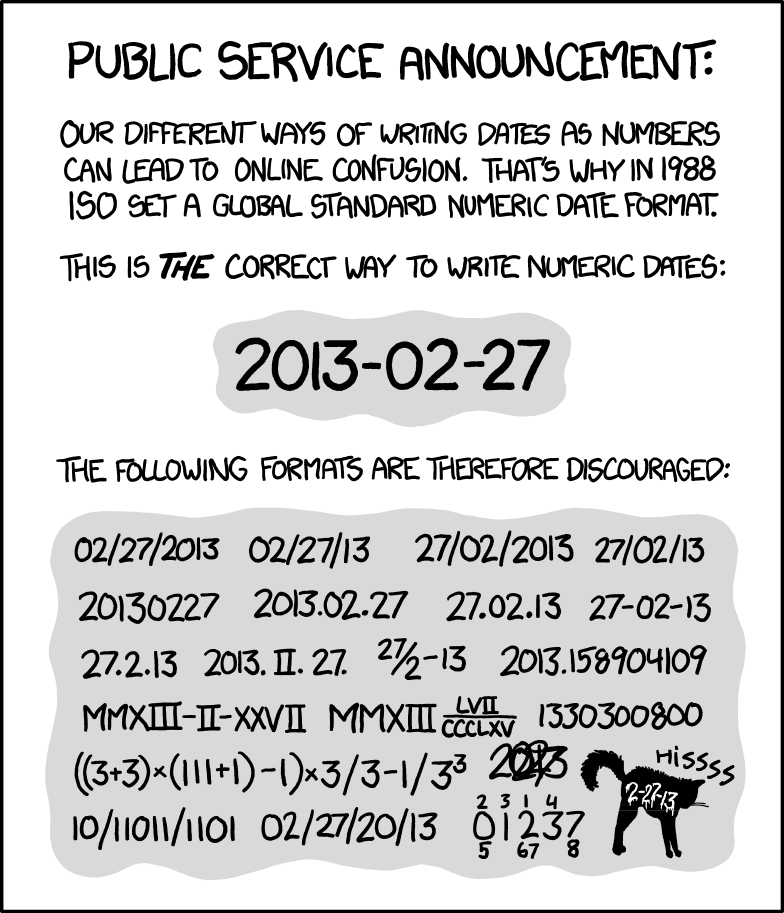
\includegraphics[width=10.89in]{images/iso_8601_2x}

\href{https://xkcd.com/1179/}{ISO 8601 -- xkcd}

\hypertarget{final-project}{%
\section{Final Project}\label{final-project}}

There is a final project in place of a final exam for this class. You will find your own dataset that helps you answer a question that you're interested in. You'll bring these data into R, explore it, clean it, make features, and run an analysis that allows you to answer your question. You will be graded on the completed R script as well as your presentation of the data.

The presentation will last 3-4 minutes, and will take place on the day of the final exam (in place of the exam). University policy on final examinations can be found here: \url{https://www.registrar.arizona.edu/courses/final-examination-regulations-and-information}

\hypertarget{honors-students-requirements}{%
\section{Honors Students' Requirements}\label{honors-students-requirements}}

Students wishing to take this course for Honors Credit should email me to set up an appointment to discuss the terms of the contact and to sign the Honors Course Contract Request Form. The form is available at \url{https://honors.arizona.edu/academics/honors-contracts}. Students earning credit with the University of Arizona Honors College will be held to the following enhancements:

\begin{enumerate}
\def\labelenumi{\arabic{enumi}.}
\item
  Honors students will be required to create an academic poster based on their final project, and then present this poster at the iSchool's iShowcase at the end of the semester. Creating a poster will require extra work to ensure clarity of logic, having a well-defined question and approach, and the creation of quality visuals. Guidelines on how to create an engaging academic poster can be found here: \url{https://guides.nyu.edu/posters}. Note: The iShowcase is at the end of the semester, but before finals when the regular class will have the project due. Thus, you will have to be ahead of schedule a bit to meet your honors requirement.
\item
  Honors students will also be expected to informally `journal' about the course each week. Each week, that is, students will be required to write a five-sentence paragraph reflecting on some issue or moment that has arisen in our readings or discussions (e.g., the problem with particular terms or some philosophical or practical dilemma). Ultimately, if offering a paragraph each week, honors students will have written roughly 15 reflective paragraphs for the semester. This must be emailed directly to me by Sunday 5pm each week.
\end{enumerate}

\hypertarget{student-accommodations}{%
\section{Student Accommodations}\label{student-accommodations}}

It is the University's goal that learning experiences be as accessible as possible. If you anticipate or experience physical or academic barriers based on disability or pregnancy, please let me know immediately so that we can discuss options. You are also welcome to contact Disability Resources (520-621-3268) to establish reasonable accommodations. For additional information on Disability Resources and reasonable accommodations, please visit \url{http://drc.arizona.edu/}.

\hypertarget{attendance-due-dates-and-missing-work}{%
\section{Attendance, Due Dates, and Missing Work}\label{attendance-due-dates-and-missing-work}}

\begin{enumerate}
\def\labelenumi{\arabic{enumi}.}
\tightlist
\item
  Missed class assignments or exams cannot be made up without a well-documented, verifiable, excuse (for example, a physician's medical excuse). Indeed, due dates are firm, and late work will be accepted only with a verifiable and valid excuse.
\item
  The UA policy regarding absences for any sincerely held religious belief, observance or practice will be accommodated where reasonable, \url{http://policy.arizona.edu/human-resources/religious-accommodation-policy}.
\item
  Absences pre-approved by the UA Dean of Students (or Dean designee) will be honored. \url{https://deanofstudents.arizona.edu/absences}\\
\item
  Arriving late and leaving early is extremely disruptive to others in the class. Please avoid this kind of disruption.
\item
  The UA's policy concerning Class Attendance and Administrative Drops is available at: \url{https://catalog.arizona.edu/policy/class-attendance-participation-and-administrative-drop}
\end{enumerate}

\hypertarget{course-conduct-and-campus-policies}{%
\section{Course Conduct and Campus Policies}\label{course-conduct-and-campus-policies}}

It's important to be familiar with all campus policies.

\begin{enumerate}
\def\labelenumi{\arabic{enumi}.}
\item
  Students are encouraged to share intellectual views and discuss freely the principles and applications of course materials. However, graded work/exercises must be the product of independent effort unless otherwise instructed. Students are expected to adhere to the UA Code of Academic Integrity as described in the UA General Catalog. See: \url{http://deanofstudents.arizona.edu/academic-integrity/students/academic-integrity}.
\item
  It is the University's goal that learning experiences be as accessible as possible. If you anticipate or experience physical or academic barriers based on disability or pregnancy, please let me know immediately so that we can discuss options. You are also welcome to contact Disability Resources (520-621-3268) to establish reasonable accommodations. For additional information on Disability Resources and reasonable accommodations, please visit \url{http://drc.arizona.edu/}.
\item
  The UA Threatening Behavior by Students Policy prohibits threats of physical harm to any member of the University community, including to oneself. See \url{http://policy.arizona.edu/education-and-student-affairs/threatening-behavior-students}.
\item
  All student records will be managed and held confidentially. \url{http://www.registrar.arizona.edu/personal-information/family-educational-rights-and-privacy-act-1974-ferpa?topic=ferpa}
\item
  The University is committed to creating and maintaining an environment free of discrimination; see \url{http://policy.arizona.edu/human-resources/nondiscrimination-and-anti-harassment-policy}.
\item
  Information contained in this syllabus, other than the grade and absence policy, may be subject to change without advance notice as deemed appropriate by the instructor.
\end{enumerate}

\hypertarget{code-of-conduct}{%
\section{Code of Conduct}\label{code-of-conduct}}

This code of conduct is based on \href{https://docs.github.com/en/github/site-policy/github-community-guidelines}{GitHub Community Guidelines}. One of the goals of this course is to get you familiar with the data science community, and how people work and learn better together. This is a community we build together, and we need everybody's help to make it better each day.

\hypertarget{our-pledge}{%
\subsection{Our Pledge}\label{our-pledge}}

In the interest of fostering an open and welcoming environment, we as instructor and students pledge to making participation in our community a harassment-free experience for everyone, regardless of age, body size, disability, ethnicity, gender identity and expression, level of experience, nationality, personal appearance, race, religion, or sexual identity and orientation.

\begin{itemize}
\item
  \textbf{Be welcoming and open-minded.} Although this is an intro course, like in any other learning setting, we have people at different levels of experience. Other people may not have the same experience level or background as you, but that doesn't mean they don't have good ideas to contribute. I encourage you to be welcoming to everyone, from more advanced coders to those just getting started. We can all learn from each other.
\item
  \textbf{Respect each other.} Nothing sabotages healthy conversation like rudeness. Be civil and professional, and don't post or say anything that a reasonable person would consider offensive, abusive, or hate speech. Don't harass or grief anyone. Treat each other with dignity and consideration in all interactions.
\end{itemize}

You may wish to respond to something by disagreeing with it. That's fine. But remember to criticize ideas, not people. Avoid name-calling, ad hominem attacks, responding to a post's tone instead of its actual content, and knee-jerk reactions. Instead, provide reasoned counter-arguments that improve the conversation.

\begin{itemize}
\item
  \textbf{Communicate with empathy.} Disagreements or differences of opinion are a fact of life. Being part of a community means interacting with people from a variety of backgrounds and perspectives (and we are all better because of this variety), many of which may not be your own. If you disagree with someone, try to understand and share their feelings before you address them. This will promote a respectful and friendly atmosphere where people feel comfortable asking questions, participating in discussions, and making contributions.
\item
  \textbf{Be clear and stay on topic.} The goal of this course is to learn about data science and how to do data science with R. Off-topic comments are a distraction (sometimes welcome, but usually not) from getting work done and being productive. Staying on topic helps produce positive and productive discussions.
\end{itemize}

Additionally, as this class will be conducted online, you might not have met each other in person. Communicating on the internet can be awkward, even when you already know people. It's hard to convey or read tone, and sarcasm is frequently misunderstood. Try to use clear language, and think about how it will be received by the other person.

\hypertarget{our-standards}{%
\subsection{Our Standards}\label{our-standards}}

Examples of behavior that contributes to creating a positive environment include:

\begin{itemize}
\item
  Using welcoming and inclusive language
\item
  Being respectful of differing viewpoints and experiences
\item
  Gracefully accepting constructive criticism
\item
  Focusing on what is best for the community
\item
  Showing empathy towards other community members
\end{itemize}

Examples of unacceptable behavior by participants include:

\begin{itemize}
\item
  The use of sexualized language or imagery and unwelcome sexual attention or advances
\item
  Trolling, insulting/derogatory comments, and personal or political attacks
\item
  Public or private harassment
\item
  Publishing others' private information, such as a physical or electronic address, without explicit permission
\item
  Other conduct which could reasonably be considered inappropriate in a professional setting
\end{itemize}

\hypertarget{enforcement}{%
\subsection{Enforcement}\label{enforcement}}

Instances of abusive, harassing, or otherwise unacceptable behavior may be reported by contacting your instructor at \href{mailto:adrianaps@email.arizona}{\nolinkurl{adrianaps@email.arizona}}. Your instructor will review and investigate all complaints, and will respond in a way that it deems appropriate to the circumstances. Your instructor is obligated to maintain confidentiality with regard to the reporter of an incident.

\hypertarget{attribution}{%
\subsection{Attribution}\label{attribution}}

This Code of Conduct is adapted from the \href{https://www.contributor-covenant.org/}{Contributor Covenant}, version 1.4, available at \url{http://contributor-covenant.org/version/1/4}

\hypertarget{how-to-ask-for-help}{%
\section{How to Ask For Help}\label{how-to-ask-for-help}}

We'll see in this course that a key skill that you should develop as a data science is the ability to find solutions to problems. Knowing how to get help is part of that skill.

\hypertarget{before-you-ask-for-help}{%
\subsection{Before You ask for help}\label{before-you-ask-for-help}}

\begin{itemize}
\item
  \textbf{Check for typos.} One of the most common causes of errors are typos, which usually throw an error such as {Error in \_\_\_\_\_ : could not find function ``\_\_\_\_\_''} due to a function being misspelled
\item
  \textbf{Check loaded packages.} You also get errors like {Error in data \%\textgreater\% summary() : could not find function ``\%\textgreater\%''} when you failed to load a package.
\item
  \textbf{Read the error message.} Don't ignore what R is telling you. Be aware that red text that appears in your console is not alwayws indication of errors. Sometimes it's just a warning.
\item
  \textbf{Google is your friend.} Copy and paste the exact error message on a Google search. (this step also includes \textbf{read the documentation} on the package you're trying to use).
\item
  If you are still stuck, you an always try \textbf{rubber duck debugging}. Describe the problem aloud, explaining it line-by-line, to a rubber duck or another person (who might not have any experience with programming of data science). This is also a good preparation step to asking other people for help (next section).
\end{itemize}

\hypertarget{ask-other-people-for-help}{%
\subsection{Ask other people for help}\label{ask-other-people-for-help}}

Like mentioned before, you should ask your peers for help before you ask your instructor. Relying on a single person to solve all of your problems is dangerous, because that person won't be available throughout your career as a data scientist.

\begin{itemize}
\item
  Check \href{https://ischool-esoc214.slack.com}{\textbf{our Slack}} to see if someone else has asked a question similar to yours, and whether there's a solution posted for it.
\item
  \textbf{Be precise and informative}. The more context you can provide about what you're trying to do and what errors you're getting, the better. Also describe the steps you took to try to solve the problem yourself.
\end{itemize}

\hypertarget{list-of-resources}{%
\subsection{List of Resources}\label{list-of-resources}}

\begin{itemize}
\tightlist
\item
  \href{https://www.r-project.org/help.html}{Getting Help with R}
\item
  \href{https://www.youtube.com/watch?v=ZFaWxxzouCY\&feature=youtu.be}{Roger Peng's How To Get Help video}
\item
  \href{https://rubberduckdebugging.com/}{Rubber Duck Debugging}
\end{itemize}

\hypertarget{whats_ds}{%
\chapter{What's data science?}\label{whats_ds}}

\hypertarget{before-class-1}{%
\section{Before class \#1}\label{before-class-1}}

Required external reading for this module: \href{readings/module2_what_is_data_science.pdf}{What's data science?} (4,660 words, approx. 20 minutes of reading time)

Watch the \href{https://youtu.be/6OFm7YcunWc?t=617}{YouTube video Angry Hiring Manager Panel} from 10:18 to 16:48 (6.5 minutes) and list the skills they mention as important to have in a data science position.

Fill out \href{https://forms.gle/NaqrC87cB8xh6Sdz8}{Survey 1} (10 min)

\hypertarget{whats-data-science}{%
\section{What's data science?}\label{whats-data-science}}

Data science is one of the fields with the highest demand, with prospects of increased demand for the next decade \citep{kross2020democratization, hadavand2018can}. Interestingly, the data scientist title was invented in 2008, and the median base salary for a data scientist surpassed \$100,000 in the United States in 2019 \citep{robinson_nolis_2020}.

\leavevmode\hypertarget{challenge}{}%
Based on your own experience and on your reading for this module, in your groups discuss the following question:

\begin{itemize}
\tightlist
\item
  What is data science?
\end{itemize}

\hypertarget{what-does-a-data-scientist-do}{%
\section{What does a data scientist do?}\label{what-does-a-data-scientist-do}}

Data science is an interdisciplinary field, and as such data scientists hold jobs with a broad range of skills, from statistics to communication. \href{https://www.google.com/search?rlz=1C5CHFA_enUS843US843\&sxsrf=ALeKk02S5o7eqMYtn1l_VE-dvUDmZjXxKw:1594738746865\&ei=OsgNX8ObNMSD9PwP6JS2gAM\&q=data+science+jobs\&oq=data+science+\&gs_lcp=CgZwc3ktYWIQAxgAMggIABCxAxCRAjIICAAQsQMQkQIyAggAMgUIABCxAzIECAAQQzICCAAyBQgAELEDMgUIABCxAzIHCAAQsQMQQzIFCAAQsQM6BAgAEEc6BQgAEJECOggIABCxAxCDAToKCAAQsQMQgwEQQ1C3S1icVWDgYGgAcAN4AIABjwGIAcwKkgEDOC41mAEAoAEBqgEHZ3dzLXdpeg\&sclient=psy-ab\&ibp=htl;jobs\&sa=X\&ved=2ahUKEwj2vc_qgM3qAhXEZs0KHTpaC8EQiYsCKAF6BAgKEBA\#htivrt=jobs\&htidocid=cxgsZF4SHt5PJepoAAAAAA\%3D\%3D\&fpstate=tldetail}{A quick Google search for data science jobs} reveals this long list of skills. However, no single data scientist has all skills listed for different data science jobs. Instead, each data scientist specializes in different skills \citep{robinson_nolis_2020}.

\leavevmode\hypertarget{challenge}{}%
Make a list of skills listed on data science job announcements and in the video you just watched. Based on these, discuss the following questions in your group:

\begin{enumerate}
\def\labelenumi{\arabic{enumi})}
\item
  Which skills do you already have? At what level of proficiency?
\item
  Which skills are you interested in developing further?
\item
  Based on the skills you already have, and the skills you want to acquire, what type of job in data science would you be interested in?
\end{enumerate}

\hypertarget{data-science-workflow}{%
\section{Data Science Workflow}\label{data-science-workflow}}

The basic data science workflow involve three main parts:

\begin{enumerate}
\def\labelenumi{\arabic{enumi})}
\item
  The Question: Form the question you want to answer. Many times you will be given a question, and you have to ``translate'' it so you can answer it with your data analysis.
\item
  Data Acquisition: data file, database, or web API
\item
  Data Wrangling: import + tidy data + transform \citep{grolemund2018r}
\item
  Data Exploration: transform + visualize + model + repeat \citep{grolemund2018r}
\item
  Results Communication: visualize + write + knit \citep{grolemund2018r}
\end{enumerate}

\begin{figure}

{\centering 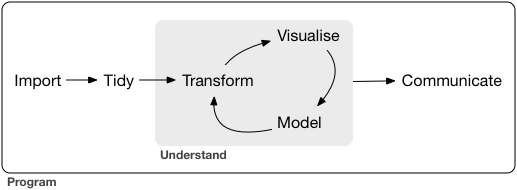
\includegraphics[width=0.5\linewidth]{images/data-science} 

}

\caption{typical data science project model (Grolemund and Wickham, 2018)}\label{fig:unnamed-chunk-3}
\end{figure}

\leavevmode\hypertarget{challenge}{}%
In your groups, based on your own intuition and experience, and based on the \href{https://r4ds.had.co.nz/introduction.html}{Introduction to R for Data Science} book \citep{grolemund2018r}, summarize what each of the following steps means:

\begin{enumerate}
\def\labelenumi{\arabic{enumi})}
\item
  Tidy
\item
  Transform
\item
  Visualize
\item
  Model
\item
  Communicate
\end{enumerate}

We will approach the entire data science workflow in this course (but not necessarily every step listed), not in this order. We start with step 3 (Data Wrangling) and 4 (Data Exploration), before we address step 2 (Data Acquisition) and step 5 (Communication)

\leavevmode\hypertarget{challenge}{}%
Go back to the list of skills and job positions we discussed (based on the reading and the video):

\begin{enumerate}
\def\labelenumi{\arabic{enumi})}
\tightlist
\item
  Which steps in the data science workflow correspond to the job skills we talked about?
\end{enumerate}

\hypertarget{before-class-2}{%
\section{Before class \#2}\label{before-class-2}}

Please fill out \href{https://forms.gle/NaqrC87cB8xh6Sdz8}{Survey 1} (10 min).

Reading: \href{readings/module2_eds_leek_whatsdatascience.pdf}{Data Science examples} (1,0333 words, 8 min)

Reading: \href{readings/module2_modern_data_science_data_intake.pdf}{Data Intake} (1,686 words, 12 min)

\hypertarget{whats-data}{%
\section{What's data?}\label{whats-data}}

\leavevmode\hypertarget{challenge}{}%
In your small group, discuss the examples provided in the excerpt from ``Executive Data Science'' \citep{caffo2016executive}.

\begin{enumerate}
\def\labelenumi{\arabic{enumi})}
\item
  How is this definition of Data Science different from other definitions we discussed so far?
\item
  Why did Netflix end up not implementing the best solution from the Netflix prize challenge?
\item
  What data was used in each of the examples provided?
\item
  What is data? (come up with a definition).
\end{enumerate}

~

Examples of what data might look like.

\begin{itemize}
\tightlist
\item
  Structured data (rare):
\end{itemize}

State

School Year

Average Tuition

Nevada

2004-05

3621.392

Nevada

2005-06

3687.290

Florida

2004-05

3848.201

Florida

2007-08

3879.416

Florida

2006-07

3887.656

Florida

2005-06

3924.234

Wyoming

2008-09

3928.671

Wyoming

2007-08

4071.898

Wyoming

2004-05

4086.351

Wyoming

2006-07

4122.205

\leavevmode\hypertarget{challenge}{}%
Which of the columns (or variables) in the data frame above are \textbf{categorical}, which are \textbf{quantitative}?

;nbsp

\begin{itemize}
\tightlist
\item
  Structured, but messy data (more common):
\end{itemize}

State

2004-05

2005-06

2006-07

2007-08

2008-09

2009-10

2010-11

2011-12

2012-13

2013-14

2014-15

2015-16

Alabama

5682.838

5840.550

5753.496

6008.169

6475.092

7188.954

8071.134

8451.902

9098.069

9358.929

9496.084

9751.101

Alaska

4328.281

4632.623

4918.501

5069.822

5075.482

5454.607

5759.153

5762.421

6026.143

6012.445

6148.808

6571.340

Arizona

5138.495

5415.516

5481.419

5681.638

6058.464

7263.204

8839.605

9966.716

10133.503

10296.200

10413.844

10646.278

Arkansas

5772.302

6082.379

6231.977

6414.900

6416.503

6627.092

6900.912

7028.991

7286.580

7408.495

7606.410

7867.297

California

5285.921

5527.881

5334.826

5672.472

5897.888

7258.771

8193.739

9436.426

9360.574

9274.193

9186.824

9269.844

Colorado

4703.777

5406.967

5596.348

6227.002

6284.137

6948.473

7748.201

8315.632

8792.856

9292.954

9298.599

9748.188

Connecticut

7983.695

8249.074

8367.549

8677.702

8720.976

9371.019

9827.013

9736.431

10036.627

10453.110

10663.995

11397.337

Delaware

8352.890

8610.597

8681.846

8945.801

8995.473

9987.183

10534.181

11026.241

11362.690

11502.524

11514.660

11676.216

Florida

3848.201

3924.234

3887.656

3879.416

4150.004

4783.032

5510.659

5940.945

6494.901

6451.664

6345.000

6360.159

Georgia

4298.040

4492.167

4584.268

4790.266

4831.365

5549.913

6428.007

7709.284

7853.257

7992.390

8063.014

8446.961

\begin{center}\rule{0.5\linewidth}{0.5pt}\end{center}

user\_id

screen\_name

text

reply\_to\_screen\_name

6.331283e+07

blagogirl

\citet{realTuckFrumper} The illiterate calling Iran out?
80 million bounty on Trumps head?

realTuckFrumper

6.331283e+07

blagogirl

\citet{JonHutson} Iran does NOT fear Trump.
They realize what OUR country is dealing with.
``The White House is inflicted with mental retardation''

JonHutson

1.125104e+18

dl\_kirkwood

I'm afraid 11 soldiers had to be shipped out from the Iran hit after all with traumatic brain injuries. Seems the Military does not notify homeland unless a soldiers is shipped out for the injury. So, Trump did not know for a week. \url{https://t.co/HdBNbKClBl}

NA

2.820552e+07

djbarro

\citet{GloriaAllred} Are you going to carry a sign supporting the women in Iran brave enough to remove their hijabs and go to prison?

GloriaAllred

1.506314e+08

kizu91

US\ldots Special\ldots Representative\ldots Hold\ldots Press\ldots Briefing\ldots Situation in\ldots Iran\ldots Video\ldots first\ldots week\ldots January\ldots saw\ldots drastic\ldots spike\ldots tensions\ldots Washington\ldots Tehran\ldots President\ldots Donald Trump\ldots order\ldots assassination\ldots elite\ldots Quds\ldots Force\ldots commander\ldots Qasem\ldots Soleimani\ldots Iraq

NA

1.506314e+08

kizu91

crash\ldots land\ldots collide\ldots plane\ldots aircraft\ldots all\ldots176\ldots people\ldots on board\ldots Iran\ldots missile\ldots attack\ldots US\ldots base\ldots Iraq\ldots rocket\ldots Western\ldots Sahara\ldots Suriname\ldots Colombia\ldots Dominica\ldots Australia\ldots Anguilla\ldots Guadeloupe\ldots Uruguay\ldots Cyprus\ldots Namibia\ldots Brazil\ldots Paraguay\ldots Denmark\ldots55

NA

1.506314e+08

kizu91

Iran\ldots MP\ldots Urge\ldots Gov't\ldots Expel\ldots UK\ldots Envoy\ldots Consider\ldots Downgrading\ldots Diplomatic\ldots Ties\ldots Alleged\ldots Meddling\ldots envoy\ldots Robert Macaire\ldots detained\ldots days\ldots ago\ldots alleged\ldots participation\ldots unsanctioned\ldots protest\ldots Tehran\ldots down\ldots Ukraine\ldots Boeing\ldots737\ldots release\ldots15\ldots minutes

NA

1.506314e+08

kizu91

Government\ldots Supporter\ldots Gather\ldots Tehran\ldots13\ldots.Friday\ldots Prayer\ldots Video\ldots Iran\ldots gather\ldots rally\ldots commemorate\ldots kill\ldots fatal\ldots crash\ldots land\ldots collide\ldots Ukraine\ldots Boeing\ldots plane\ldots aircraft\ldots shot\ldots down\ldots missile\ldots rocket\ldots January\ldots Imam\ldots Khomeini\ldots International\ldots Airport\ldots16

NA

1.506314e+08

kizu91

British\ldots Treasury\ldots Expand\ldots Hezbollah\ldots Asset\ldots Freeze\ldots UK\ldots government\ldots approved\ldots measure\ldots follow\ldots heat\ldots conflict\ldots United States\ldots Islamic\ldots Republic\ldots Iran\ldots Trump\ldots Administration\ldots target\ldots assassination\ldots high-profile\ldots military\ldots general\ldots early\ldots January\ldots film

NA

7.297365e+17

SwmpladySH

Hackers Are Coming for the 2020 Election --- And We're Not Ready \url{https://t.co/q82kNu9gMd} via \citet{RollingStone}

NA

\begin{itemize}
\tightlist
\item
  Textual Data (always messy):
\end{itemize}

\begin{verbatim}
##  [1] "CHAPTER I"                                                               
##  [2] ""                                                                        
##  [3] ""                                                                        
##  [4] "Emma Woodhouse, handsome, clever, and rich, with a comfortable home"     
##  [5] "and happy disposition, seemed to unite some of the best blessings of"    
##  [6] "existence; and had lived nearly twenty-one years in the world with very" 
##  [7] "little to distress or vex her."                                          
##  [8] ""                                                                        
##  [9] "She was the youngest of the two daughters of a most affectionate,"       
## [10] "indulgent father; and had, in consequence of her sister's marriage, been"
\end{verbatim}

\leavevmode\hypertarget{challenge}{}%
What data formats are out there in the world. Create a list based on your experience and the excerpt from ``Modern Data Science with R'' \citep{baumer2017modern}.

\hypertarget{what-does-data-analysis-look-like}{%
\section{What does data analysis look like?}\label{what-does-data-analysis-look-like}}

The way you communicate your data analysis will depend on what question you're trying to answer and who your audience is. Here are some of my favorite data analysis reports:

\begin{itemize}
\item
  \href{https://twitter.com/IsChiaThere/status/1282681472185401349/photo/1}{Whose (coffee) beans reign supreme?} A \#tidytuesday static image
\item
  \href{https://twitter.com/geokaramanis/status/1283410776913514496/photo/1}{Women in Space} A \#tidytuesday static image
\item
  \href{https://sebastianwolf.shinyapps.io/stravachaserapp/}{Which city is faster?} A City Cycle Race Shinny app
\item
  \href{https://pudding.cool/2020/07/gendered-descriptions/}{The Physical Traits that Define Men and Women in Literature} An interactice website
\end{itemize}

\hypertarget{install-r}{%
\chapter{Exploring our IDE (Rstudio)}\label{install-r}}

\hypertarget{before-class}{%
\section{Before class}\label{before-class}}

Install R and RStudio.

We are using RStudio as our IDE for this course. If you are running your R code in your computer, you need to install both R and RStudio. Alternatively, you can create a free account at \url{http://rstudio.cloud} and run your R code in the cloud. Either way, we will be using the same IDE (i.e., RStudio).

\leavevmode\hypertarget{explanation}{}%
What's an \textbf{IDE}? IDE stands for \textbf{i}ntegrated \textbf{d}evelopment \textbf{e}nvironment, and its goal is to facilitate coding by integrating a \textbf{text editor}, a \textbf{console} and other tools into one window.

\hypertarget{ive-never-installed-r-and-rstudio-in-my-computer-or-im-not-sure-i-have-r-and-rstudio-installed-in-my-computer}{%
\subsection{I've never installed R and RStudio in my computer OR I'm not sure I have R and RStudio installed in my computer}\label{ive-never-installed-r-and-rstudio-in-my-computer-or-im-not-sure-i-have-r-and-rstudio-installed-in-my-computer}}

\begin{enumerate}
\def\labelenumi{\arabic{enumi}.}
\tightlist
\item
  Download and install R from \url{https://cran.r-project.org} (If you are a Windows user, first \href{https://www.computerhope.com/issues/ch001121.htm\#:~:text=Press\%20and\%20hold\%20the\%20Windows,running\%20the\%2064\%2Dbit\%20version.}{determine if you are running the 32 or the 64 bit version})
\item
  Download and install RStudio from \url{https://rstudio.com/products/rstudio/download/\#download}
\end{enumerate}

Here's a \href{https://youtu.be/Iwp8bm7w4fQ}{video on how to install R and RStudio on a mac}.

\hypertarget{i-already-have-r-and-rstudio-installed}{%
\subsection{I already have R and RStudio installed}\label{i-already-have-r-and-rstudio-installed}}

\begin{enumerate}
\def\labelenumi{\arabic{enumi}.}
\tightlist
\item
  Open RStudio
\item
  Check your R version by entering \texttt{sessionInfo()} on your console.
\item
  The latest release for R was June 22, 2020 (R version 4.0.2 Taking Off Again). If your R version is older than the most recent version, please follow step 1 in the previous section to update R.
\item
  Check your RStudio version, if your version is older than Version 1.3.x, please follow step 2 in the previous section to update RStudio.
\end{enumerate}

\leavevmode\hypertarget{explanation}{}%
How often should I update R and RStudio? Always make sure that you have the latest version of R, RStudio, and the packages you're using in your code to ensure you are not running into bugs that are caused by having older versions installed in your computer.

When \href{https://community.rstudio.com/t/should-i-update-all-my-r-packages-frequently-yes-no-why/5856/4}{asked}, \href{https://community.rstudio.com/u/jennybryan}{Jenny Bryan} summarizes the importance of keeping your system up-to-date saying that ``You will always eventually have a reason that you must update. So you can either do that very infrequently, suffer with old versions in the middle, and experience great pain at update. Or admit that maintaining your system is a normal ongoing activity, and do it more often.''

~

You can ensure your packages are also up-to-date by clicking on ``Tools'' on your RStudio top menu bar, and selecting ``Check for Packages Updates\ldots{}''

\hypertarget{why-learn-r}{%
\section{Why learn R?}\label{why-learn-r}}

R is both a programming language and \href{https://www.r-project.org/}{a free software environment for statistical computing and graphics}. In addition to being free, here are other reasons to learn R:

\begin{itemize}
\item
  \textbf{R is popular.} According to \href{http://r4stats.com/articles/popularity/}{Robert A. Muenchen's post on the popularity of data science software} (which is updated frequently), R is among the top 5 technologies that are mentioned in data science job ads on indeed.com.
\item
  \textbf{R is very powerful and versatile}. From creating websites (like this bookdown you're reading right now) to building machine learning models, R has it all.
\item
  \textbf{The R community is active and very supportive}. Because R is so popular, there are a number of forums on R. A good way to get a glimpse on how active the R community is to follow \href{https://twitter.com/search?q=\%23rstats}{\texttt{\#rstats}} on twitter.
\end{itemize}

\hypertarget{why-use-rstudio}{%
\section{Why use RStudio?}\label{why-use-rstudio}}

You can just use R, but RStudio is an IDE that makes using R easier and more fun. Some features that make RStudio the IDE that many data scientists use:

\begin{itemize}
\item
  RStudio is \textbf{free} and \textbf{open source}.
\item
  RStudio contains a full-feature integrated text editor, with tab-completion, spellcheck, etc.
\item
  RStudio is a cross-platform interface that looks the same across platforms.
\item
  RStudio allows you to organize your data science projects so you're not always hunting for the right script that goes with the data you want to analyze. (also, it integrates nicely with \texttt{rmarkdown} and \texttt{knitr})
\end{itemize}

\hypertarget{create-an-r-project}{%
\section{Create an R Project}\label{create-an-r-project}}

In today's class, we will focus on situating ourselves around our IDE. For every lesson, we will either start a new R project or open an R project we've been working on.

Why create a RStudio project? RStudio projects make it easier to keep your projects organized, since each project has their own working directory, workspace, history, and source documents. In other words, it's much easier to open an R project and not have to worry about setting your working directory than to try to hunt down your files.

\leavevmode\hypertarget{steps}{}%
Here are the steps we are starting with today:

\begin{enumerate}
\def\labelenumi{\arabic{enumi}.}
\item
  Start a new R project
\item
  Create a new R script
\item
  Save that R script as 01-class\_one
\end{enumerate}

~

\leavevmode\hypertarget{challenge}{}%
Take a moment to look around your IDE. What are the main panes on the RStudio interface. What are the 4 main areas of the interface? Can you guess what each area is for?

\hypertarget{operations-and-objects}{%
\section{Operations and Objects}\label{operations-and-objects}}

Let's start by using R as a calculator. On your \textbf{console} type \texttt{3\ +\ 3} and hit enter.

\begin{Shaded}
\begin{Highlighting}[]
\DecValTok{3} \OperatorTok{+}\StringTok{ }\DecValTok{3}
\end{Highlighting}
\end{Shaded}

\begin{verbatim}
## [1] 6
\end{verbatim}

\leavevmode\hypertarget{question}{}%
What symbols do we use for all basic operations (addition, subtraction, multiplication, and division)?
What happens if you type \texttt{3\ +}?

Let's save our calculation into an object, by using the assignment symbol \texttt{\textless{}-}.

\begin{Shaded}
\begin{Highlighting}[]
\NormalTok{sum_result <-}\StringTok{ }\DecValTok{3} \OperatorTok{+}\StringTok{ }\DecValTok{3}
\end{Highlighting}
\end{Shaded}

\leavevmode\hypertarget{question}{}%
Take a moment to look around your IDE once again. What has changed?

Now, let's use this new object in our calculation

\begin{Shaded}
\begin{Highlighting}[]
\NormalTok{sum_result }\OperatorTok{+}\StringTok{ }\DecValTok{3}
\end{Highlighting}
\end{Shaded}

\begin{verbatim}
## [1] 9
\end{verbatim}

\leavevmode\hypertarget{question}{}%
Take a moment to look around your IDE once again. Has anything changed?

What else can we do with an object?

\begin{Shaded}
\begin{Highlighting}[]
\KeywordTok{class}\NormalTok{(sum_result)}
\end{Highlighting}
\end{Shaded}

\begin{verbatim}
## [1] "numeric"
\end{verbatim}

R is primarily a functional programming language. That means that there pre-programmed functions in base R such as \texttt{class()} and that you can also write your own functions (more on that later).

Type \texttt{?class} in your console and hit enter to get more information about this function.

\leavevmode\hypertarget{challenge}{}%
CHALLENGE

Create an object called \texttt{daisys\_age} that holds the number 8.
Multiply \texttt{daisys\_age} by 4 and save the results in another object called \texttt{daisys\_human\_age}

Imagine I had multiple pets (unfortunately, that is not true, Daisy is my only pet). I can create a \textbf{vector} to hold multiple numbers representing the age of each of my pets.

\begin{Shaded}
\begin{Highlighting}[]
\NormalTok{my_pets_ages <-}\StringTok{ }\KeywordTok{c}\NormalTok{(}\DecValTok{8}\NormalTok{, }\DecValTok{2}\NormalTok{, }\DecValTok{6}\NormalTok{, }\DecValTok{3}\NormalTok{, }\DecValTok{1}\NormalTok{)}
\end{Highlighting}
\end{Shaded}

\leavevmode\hypertarget{question}{}%
Take a moment to look around your IDE once again. What has changed?

What is the class of the object \texttt{my\_pets\_ages}?

Now let's multiply this vector by 4.

\begin{Shaded}
\begin{Highlighting}[]
\NormalTok{my_pets_ages }\OperatorTok{*}\StringTok{ }\DecValTok{4}
\end{Highlighting}
\end{Shaded}

\begin{verbatim}
## [1] 32  8 24 12  4
\end{verbatim}

Errors are pretty common when writing code in any programming language, so be ready to read error messages and debug your code. Let's insert a typing error in our previous code:

\begin{Shaded}
\begin{Highlighting}[]
\NormalTok{my_pets_ages <-}\StringTok{ }\KeywordTok{c}\NormalTok{(}\DecValTok{8}\NormalTok{, }\DecValTok{2}\NormalTok{, }\DecValTok{6}\NormalTok{, }\StringTok{'3'}\NormalTok{, }\DecValTok{1}\NormalTok{)}
\end{Highlighting}
\end{Shaded}

\leavevmode\hypertarget{challenge}{}%
CHALLENGE

Try to multiply \texttt{my\_pets\_ages} by 4. What happens? How can we debug our code to find out what is causing the error?

\hypertarget{r-basics}{%
\chapter{R Basics}\label{r-basics}}

\hypertarget{before-class-3}{%
\section{Before Class}\label{before-class-3}}

Read \href{http://varianceexplained.org/programming/bad-code/}{A Million Lines of Bad Code} a blog post by \href{http://varianceexplained.org/about/}{David Robinson}. (549 words, 5 minutes)

Read \href{readings/module7_eds_whats_stats.pdf}{What is Statistics Good For?} (398 words, 3 min)

\hypertarget{dataframes}{%
\section{Dataframes}\label{dataframes}}

You will rarely work with individual numeric values, or even individual numeric vectors. Often, we have information organized in dataframes, which is R's version of a spreadsheet.

Let's go back to my imaginary pet's ages (make sure you have the correct vector in your global environment).

\begin{Shaded}
\begin{Highlighting}[]
\NormalTok{my_pets_ages <-}\StringTok{ }\KeywordTok{c}\NormalTok{(}\DecValTok{8}\NormalTok{, }\DecValTok{2}\NormalTok{, }\DecValTok{6}\NormalTok{, }\StringTok{'3'}\NormalTok{, }\DecValTok{1}\NormalTok{)}
\NormalTok{my_pets_ages <-}\StringTok{ }\KeywordTok{as.numeric}\NormalTok{(my_pets_ages)}
\end{Highlighting}
\end{Shaded}

We will now create a vector of strings or characters that holds my imaginary pets' names (we have to be careful to keep the same order then the \texttt{my\_pets\_ages} vector).

\begin{Shaded}
\begin{Highlighting}[]
\NormalTok{my_pets_names <-}\StringTok{ }\KeywordTok{c}\NormalTok{(}\StringTok{'Daisy'}\NormalTok{, }\StringTok{'Violet'}\NormalTok{, }\StringTok{'Lily'}\NormalTok{, }\StringTok{'Iris'}\NormalTok{, }\StringTok{'Poppy'}\NormalTok{)}
\end{Highlighting}
\end{Shaded}

Let's now create a dataframe that contains info about my pets.

\begin{Shaded}
\begin{Highlighting}[]
\CommentTok{# create dataframe}
\NormalTok{my_pets <-}\StringTok{ }\KeywordTok{data.frame}\NormalTok{(}\DataTypeTok{name =}\NormalTok{ my_pets_names, }\DataTypeTok{age =}\NormalTok{ my_pets_ages)}

\CommentTok{# print out dataframe}
\NormalTok{my_pets}
\end{Highlighting}
\end{Shaded}

\begin{verbatim}
##     name age
## 1  Daisy   8
## 2 Violet   2
## 3   Lily   6
## 4   Iris   3
## 5  Poppy   1
\end{verbatim}

\leavevmode\hypertarget{challenge}{}%
CHALLENGE

There's a number of functions you can run on dataframes. Try running the following functions on \texttt{my\_pets}:

\begin{itemize}
\item
  summary()
\item
  nrow()
\item
  ncol()
\item
  dim()
\end{itemize}

What other functions can/do you think/know of?

\hypertarget{slicing-you-dataframe}{%
\section{Slicing you dataframe}\label{slicing-you-dataframe}}

There are different ways you can slice or subset your dataframe.

You can use indices for rows and columns.

\begin{Shaded}
\begin{Highlighting}[]
\NormalTok{my_pets[}\DecValTok{1}\NormalTok{,]}
\end{Highlighting}
\end{Shaded}

\begin{verbatim}
##    name age
## 1 Daisy   8
\end{verbatim}

\begin{Shaded}
\begin{Highlighting}[]
\NormalTok{my_pets[, }\DecValTok{1}\NormalTok{]}
\end{Highlighting}
\end{Shaded}

\begin{verbatim}
## [1] "Daisy"  "Violet" "Lily"   "Iris"   "Poppy"
\end{verbatim}

\begin{Shaded}
\begin{Highlighting}[]
\NormalTok{my_pets[}\DecValTok{1}\NormalTok{, }\DecValTok{1}\NormalTok{]}
\end{Highlighting}
\end{Shaded}

\begin{verbatim}
## [1] "Daisy"
\end{verbatim}

You can use a column name or a row name instead of an index.

\begin{Shaded}
\begin{Highlighting}[]
\NormalTok{my_pets[, }\StringTok{'age'}\NormalTok{]}
\end{Highlighting}
\end{Shaded}

\begin{verbatim}
## [1] 8 2 6 3 1
\end{verbatim}

\begin{Shaded}
\begin{Highlighting}[]
\NormalTok{my_pets[}\StringTok{'1'}\NormalTok{, ]}
\end{Highlighting}
\end{Shaded}

\begin{verbatim}
##    name age
## 1 Daisy   8
\end{verbatim}

\begin{Shaded}
\begin{Highlighting}[]
\NormalTok{my_pets[}\StringTok{'1'}\NormalTok{, }\StringTok{'age'}\NormalTok{]}
\end{Highlighting}
\end{Shaded}

\begin{verbatim}
## [1] 8
\end{verbatim}

Or you can use \texttt{\$} to retrieve values from a column.

\begin{Shaded}
\begin{Highlighting}[]
\NormalTok{my_pets}\OperatorTok{$}\NormalTok{age}
\end{Highlighting}
\end{Shaded}

\begin{verbatim}
## [1] 8 2 6 3 1
\end{verbatim}

\begin{Shaded}
\begin{Highlighting}[]
\NormalTok{my_pets}\OperatorTok{$}\NormalTok{age[}\DecValTok{1}\NormalTok{]}
\end{Highlighting}
\end{Shaded}

\begin{verbatim}
## [1] 8
\end{verbatim}

You can also use comparisons to filter your dataframe

\begin{Shaded}
\begin{Highlighting}[]
\CommentTok{# get index with which() function}
\KeywordTok{which}\NormalTok{(my_pets}\OperatorTok{$}\NormalTok{age }\OperatorTok{==}\StringTok{ }\DecValTok{8}\NormalTok{)}
\end{Highlighting}
\end{Shaded}

\begin{verbatim}
## [1] 1
\end{verbatim}

\begin{Shaded}
\begin{Highlighting}[]
\CommentTok{# use which() inside dataframe indexing my_pets[row_number, column_number]}
\NormalTok{my_pets[}\KeywordTok{which}\NormalTok{(my_pets}\OperatorTok{$}\NormalTok{age }\OperatorTok{==}\StringTok{ }\DecValTok{8}\NormalTok{),]}
\end{Highlighting}
\end{Shaded}

\begin{verbatim}
##    name age
## 1 Daisy   8
\end{verbatim}

\begin{Shaded}
\begin{Highlighting}[]
\NormalTok{my_pets[}\KeywordTok{which}\NormalTok{(my_pets}\OperatorTok{$}\NormalTok{age }\OperatorTok{==}\StringTok{ }\DecValTok{8}\NormalTok{), }\DecValTok{1}\NormalTok{]}
\end{Highlighting}
\end{Shaded}

\begin{verbatim}
## [1] "Daisy"
\end{verbatim}

\begin{Shaded}
\begin{Highlighting}[]
\NormalTok{my_pets[}\KeywordTok{which}\NormalTok{(my_pets}\OperatorTok{$}\NormalTok{age }\OperatorTok{==}\StringTok{ }\DecValTok{8}\NormalTok{), }\StringTok{'name'}\NormalTok{]}
\end{Highlighting}
\end{Shaded}

\begin{verbatim}
## [1] "Daisy"
\end{verbatim}

\begin{Shaded}
\begin{Highlighting}[]
\NormalTok{my_pets[}\KeywordTok{which}\NormalTok{(my_pets}\OperatorTok{$}\NormalTok{age }\OperatorTok{==}\StringTok{ }\DecValTok{8}\NormalTok{),]}\OperatorTok{$}\NormalTok{name}
\end{Highlighting}
\end{Shaded}

\begin{verbatim}
## [1] "Daisy"
\end{verbatim}

\leavevmode\hypertarget{challenge}{}%
CHALLENGE

Print out a list of pet names that are older than 3.

\hypertarget{adding-new-variables-i.e.-columns-to-your-dataframe}{%
\section{Adding new variables (i.e., columns) to your dataframe}\label{adding-new-variables-i.e.-columns-to-your-dataframe}}

So far the \texttt{my\_pets} dataframe has two columns: name and age.

Let's add a third column with the pets' ages in human years. For that, we are going to use \texttt{\$} on with a variable (or column) name that does not exist in our dataframe yet. We will then assign to this variable the value in the \texttt{age} column multiplied by 4.

\begin{Shaded}
\begin{Highlighting}[]
\CommentTok{# create new column called human_years}
\NormalTok{my_pets}\OperatorTok{$}\NormalTok{human_years <-}\StringTok{ }\NormalTok{my_pets}\OperatorTok{$}\NormalTok{age }\OperatorTok{*}\StringTok{ }\DecValTok{4}

\CommentTok{# print dataframe}
\NormalTok{my_pets}
\end{Highlighting}
\end{Shaded}

\begin{verbatim}
##     name age human_years
## 1  Daisy   8          32
## 2 Violet   2           8
## 3   Lily   6          24
## 4   Iris   3          12
## 5  Poppy   1           4
\end{verbatim}

\leavevmode\hypertarget{question}{}%
Inspect the new \texttt{my\_pets} dataframe. What dimensions does it have now? How could you get a list of just the human years values in the data frame?

\hypertarget{descriptive-stats-on-dataframes}{%
\section{Descriptive stats on dataframes}\label{descriptive-stats-on-dataframes}}

Let's explore some functions for descriptive statistics.

\leavevmode\hypertarget{challenge}{}%
CHALLENGE

Try running the following functions on \texttt{my\_pets\$age} and \texttt{my\_pets\$human\_years}:

\begin{itemize}
\item
  mean()
\item
  sd()
\item
  median()
\item
  max()
\item
  min()
\item
  range()
\end{itemize}

What other functions can/do you think/know of?

\hypertarget{note-on-coding-style}{%
\section{Note on coding style}\label{note-on-coding-style}}

Coding style refers to how you name your objects and functions, how you comment your code, how you use spacing throughout your code, etc. If your coding style is consistent, your code is easier to read and easier to debug as a result. Here's some guides, so you can develop your own coding style:

\begin{itemize}
\item
  \href{https://style.tidyverse.org}{The tidyverse style guide}

  \begin{itemize}
  \item
    \href{http://adv-r.had.co.nz/Style.html}{Hadley Wickham's Advance R coding style}
  \item
    \href{https://google.github.io/styleguide/Rguide.html}{Google's R Style Guide}
  \end{itemize}
\end{itemize}

\hypertarget{organizing-data-science-projects}{%
\section{Organizing Data Science Projects}\label{organizing-data-science-projects}}

\hypertarget{intro-to-tidyverse}{%
\chapter{Intro to Tidyverse}\label{intro-to-tidyverse}}

\hypertarget{before-class-4}{%
\section{Before Class}\label{before-class-4}}

Read \href{https://www.r-bloggers.com/advice-to-young-and-old-programmers-a-conversation-with-hadley-wickham/}{Advice to Young (and Old) Programmers: A Conversation with Hadley Wickham} by Philip Waggoner (2,599 words, 10 minutes)

\hypertarget{what-are-r-packages}{%
\section{What are R Packages?}\label{what-are-r-packages}}

An R package contains functions, and it might contain data. There are a lot of R packages out here (check the Comprehensive R Archive Network, i.e., CRAN, for a \href{https://cran.r-project.org/web/packages/available_packages_by_name.html}{full list}). That is one of the beautiful things about R, anyone can create an R package to share their code.

\hypertarget{installing-packages}{%
\section{Installing Packages}\label{installing-packages}}

The function to install packages in R is \texttt{install.packages()}. We will be working with \href{https://www.tidyverse.org/}{TidyVerse} extensively in this course, which is a collection of R packages carefully designed for data science.

Open your RStudio. In your console, enter the following to install tidyverse (this may take a while).

\begin{Shaded}
\begin{Highlighting}[]
\KeywordTok{install.packages}\NormalTok{(}\StringTok{"tidyverse"}\NormalTok{)}
\end{Highlighting}
\end{Shaded}

You need to install any package only once (remember to check for new package versions and to keep your packages updated). However, with every new R session, you need to load the packages you are going to use by using the \texttt{library()} function (a library is an installed R package in your computer).

\begin{Shaded}
\begin{Highlighting}[]
\KeywordTok{library}\NormalTok{(tidyverse)}
\end{Highlighting}
\end{Shaded}

\leavevmode\hypertarget{explanation}{}%
Note that when calling the \texttt{install.packages()} function you need to enter the package name between quotation marks (e.g., ``tidyverse''). When you call the \texttt{library()} function, you don't use quotation marks (e.g., tidyverse).

\hypertarget{before-you-load-your-data}{%
\section{Before You Load your Data}\label{before-you-load-your-data}}

Although we are working within an R project, which sets the working directory automatically for you, it's good practice to check what folder you are working from by calling the \texttt{getwd()} function.

\begin{Shaded}
\begin{Highlighting}[]
\KeywordTok{getwd}\NormalTok{()}
\end{Highlighting}
\end{Shaded}

\begin{verbatim}
## [1] "/Users/adriana/Desktop/ESOC214/Fall 2020/bookdown/ESOC_214_Fall_2020"
\end{verbatim}

You can list the contents of your working directory by using the \texttt{dir()} function.

\begin{Shaded}
\begin{Highlighting}[]
\KeywordTok{dir}\NormalTok{()}
\end{Highlighting}
\end{Shaded}

We are going to create a \texttt{data} folder in our project, to keep things organized. Today we will be working with \href{https://www.kaggle.com/groundhogclub/groundhog-day}{a data set that contains groundhog day forecasts and temperature}. I cleaned up this data set already (no need for data tidying for now).

You can now list the contents of your \texttt{data} folder with the \texttt{dir()} function with a string that specifies the folder as a parameter.

\begin{Shaded}
\begin{Highlighting}[]
\KeywordTok{dir}\NormalTok{(}\StringTok{"data"}\NormalTok{)}
\end{Highlighting}
\end{Shaded}

\begin{verbatim}
## [1] "groundhog_day.csv"   "tweets.tsv"          "us_avg_tuition.xlsx"
\end{verbatim}

\hypertarget{whats-our-question-again}{%
\section{What's our question again?}\label{whats-our-question-again}}

Here's what we will focus on answering today, which is an excerpt from the \href{https://www.kaggle.com/groundhogclub/groundhog-day}{Groundhog Day Forecasts and Temperatures} kaggle page.

``Thousands gather at Gobbler's Knob in Punxsutawney, Pennsylvania, on the second day of February to await the spring forecast from a groundhog known as Punxsutawney Phil. According to legend, if Phil sees his shadow the United States is in store for six more weeks of winter weather. But, if Phil doesn't see his shadow, the country should expect warmer temperatures and the arrival of an early spring.''

So, in summary, our question is \textbf{How accurate is Punxsutawney Phil's winter weather forecast?}

\hypertarget{load-data-with-tidyverse}{%
\section{Load Data with Tidyverse}\label{load-data-with-tidyverse}}

We will use the \texttt{read\_csv()} function from the \texttt{readr} package (which is part of \texttt{tidyverse}) to read data in. Be careful, there's a similar function that is read.csv() from base R. We do want to use the function with the \texttt{\_} (i.e., \texttt{read\_csv()})

\begin{Shaded}
\begin{Highlighting}[]
\NormalTok{groundhog_predictions <-}\StringTok{ }\KeywordTok{read_csv}\NormalTok{(}\StringTok{"data/groundhog_day.csv"}\NormalTok{)}
\end{Highlighting}
\end{Shaded}

\begin{verbatim}
## Parsed with column specification:
## cols(
##   Year = col_double(),
##   Punxsutawney_Phil = col_character(),
##   February_Average_Temperature = col_double(),
##   February_Average_Temperature_Northeast = col_double(),
##   February_Average_Temperature_Midwest = col_double(),
##   February_Average_Temperature_Pennsylvania = col_double(),
##   March_Average_Temperature = col_double(),
##   March_Average_Temperature_Northeast = col_double(),
##   March_Average_Temperature_Midwest = col_double(),
##   March_Average_Temperature_Pennsylvania = col_double()
## )
\end{verbatim}

\leavevmode\hypertarget{challenge}{}%
\textbf{Reading warnings} - R often prints out warnings in red (these are not always errors). What information did you get when loading your data?

\hypertarget{inspect-your-data}{%
\section{Inspect Your Data}\label{inspect-your-data}}

As with any other programming language, there are multiple ways to doing anything. As such, there are multiple ways of inspecting your data in R. Here are some of my favorite ways of inspecting my data:

\begin{Shaded}
\begin{Highlighting}[]
\CommentTok{# get an overview of the data frame}
\KeywordTok{glimpse}\NormalTok{(groundhog_predictions)}
\end{Highlighting}
\end{Shaded}

\begin{verbatim}
## Rows: 122
## Columns: 10
## $ Year                                      <dbl> 1895, 1896, 1897, 1898, 1...
## $ Punxsutawney_Phil                         <chr> "No Record", "No Record",...
## $ February_Average_Temperature              <dbl> 26.60, 35.04, 33.39, 35.3...
## $ February_Average_Temperature_Northeast    <dbl> 15.6, 22.2, 23.6, 24.8, 1...
## $ February_Average_Temperature_Midwest      <dbl> 21.9, 33.5, 34.7, 33.3, 2...
## $ February_Average_Temperature_Pennsylvania <dbl> 17.0, 26.6, 27.9, 26.7, 2...
## $ March_Average_Temperature                 <dbl> 39.97, 38.03, 38.79, 41.0...
## $ March_Average_Temperature_Northeast       <dbl> 27.6, 25.3, 32.0, 38.0, 2...
## $ March_Average_Temperature_Midwest         <dbl> 40.2, 36.9, 44.0, 46.0, 3...
## $ March_Average_Temperature_Pennsylvania    <dbl> 31.3, 27.8, 36.9, 42.0, 3...
\end{verbatim}

\begin{Shaded}
\begin{Highlighting}[]
\KeywordTok{summary}\NormalTok{(groundhog_predictions)}
\end{Highlighting}
\end{Shaded}

\begin{verbatim}
##       Year      Punxsutawney_Phil  February_Average_Temperature
##  Min.   :1895   Length:122         Min.   :25.23               
##  1st Qu.:1925   Class :character   1st Qu.:31.78               
##  Median :1956   Mode  :character   Median :33.69               
##  Mean   :1956                      Mean   :33.80               
##  3rd Qu.:1986                      3rd Qu.:36.01               
##  Max.   :2016                      Max.   :41.41               
##  February_Average_Temperature_Northeast February_Average_Temperature_Midwest
##  Min.   :10.40                          Min.   :20.30                       
##  1st Qu.:20.02                          1st Qu.:29.62                       
##  Median :22.95                          Median :33.20                       
##  Mean   :22.69                          Mean   :32.69                       
##  3rd Qu.:25.98                          3rd Qu.:36.30                       
##  Max.   :31.60                          Max.   :41.40                       
##  February_Average_Temperature_Pennsylvania March_Average_Temperature
##  Min.   :15.20                             Min.   :35.44            
##  1st Qu.:23.60                             1st Qu.:39.38            
##  Median :26.95                             Median :41.81            
##  Mean   :26.52                             Mean   :41.70            
##  3rd Qu.:29.80                             3rd Qu.:43.56            
##  Max.   :35.80                             Max.   :50.41            
##  March_Average_Temperature_Northeast March_Average_Temperature_Midwest
##  Min.   :24.20                       Min.   :28.50                    
##  1st Qu.:29.70                       1st Qu.:39.08                    
##  Median :32.55                       Median :42.85                    
##  Mean   :32.37                       Mean   :42.57                    
##  3rd Qu.:34.80                       3rd Qu.:45.60                    
##  Max.   :43.40                       Max.   :56.30                    
##  March_Average_Temperature_Pennsylvania
##  Min.   :24.50                         
##  1st Qu.:32.95                         
##  Median :35.85                         
##  Mean   :35.91                         
##  3rd Qu.:38.55                         
##  Max.   :47.70
\end{verbatim}

\begin{Shaded}
\begin{Highlighting}[]
\CommentTok{# get variable names}
\KeywordTok{colnames}\NormalTok{(groundhog_predictions)}
\end{Highlighting}
\end{Shaded}

\begin{verbatim}
##  [1] "Year"                                     
##  [2] "Punxsutawney_Phil"                        
##  [3] "February_Average_Temperature"             
##  [4] "February_Average_Temperature_Northeast"   
##  [5] "February_Average_Temperature_Midwest"     
##  [6] "February_Average_Temperature_Pennsylvania"
##  [7] "March_Average_Temperature"                
##  [8] "March_Average_Temperature_Northeast"      
##  [9] "March_Average_Temperature_Midwest"        
## [10] "March_Average_Temperature_Pennsylvania"
\end{verbatim}

\begin{Shaded}
\begin{Highlighting}[]
\KeywordTok{names}\NormalTok{(groundhog_predictions)}
\end{Highlighting}
\end{Shaded}

\begin{verbatim}
##  [1] "Year"                                     
##  [2] "Punxsutawney_Phil"                        
##  [3] "February_Average_Temperature"             
##  [4] "February_Average_Temperature_Northeast"   
##  [5] "February_Average_Temperature_Midwest"     
##  [6] "February_Average_Temperature_Pennsylvania"
##  [7] "March_Average_Temperature"                
##  [8] "March_Average_Temperature_Northeast"      
##  [9] "March_Average_Temperature_Midwest"        
## [10] "March_Average_Temperature_Pennsylvania"
\end{verbatim}

\begin{Shaded}
\begin{Highlighting}[]
\CommentTok{# check the categorical variable}
\KeywordTok{unique}\NormalTok{(groundhog_predictions}\OperatorTok{$}\NormalTok{Punxsutawney_Phil)}
\end{Highlighting}
\end{Shaded}

\begin{verbatim}
## [1] "No Record"      "Full Shadow"    "No Shadow"      "Partial Shadow"
\end{verbatim}

\leavevmode\hypertarget{challenge}{}%
Which variables are numeric? Which are categorical?

\hypertarget{the-pipe}{%
\section{The Pipe}\label{the-pipe}}

We will be using the package \texttt{dplyr} (which is also part of \texttt{tidyverse}) to do an exploratory analysis of our data.

The package \texttt{dplyr} most used function is \texttt{\%\textgreater{}\%} (called the pipe). The pipe allows you to ``pipe'' (or redirect) objects into functions. (hint: use ctrl+shift+m or cmd+shift+m as a shortcut for typing \texttt{\%\textgreater{}\%}).

Here's how to pipe the \texttt{avocado\_data} object into the \texttt{summary()} function

\begin{Shaded}
\begin{Highlighting}[]
\CommentTok{# get an overview of the data frame}
\NormalTok{groundhog_predictions }\OperatorTok\StringTok{ }
\StringTok{  }\KeywordTok{summary}\NormalTok{()}
\end{Highlighting}
\end{Shaded}

\begin{verbatim}
##       Year      Punxsutawney_Phil  February_Average_Temperature
##  Min.   :1895   Length:122         Min.   :25.23               
##  1st Qu.:1925   Class :character   1st Qu.:31.78               
##  Median :1956   Mode  :character   Median :33.69               
##  Mean   :1956                      Mean   :33.80               
##  3rd Qu.:1986                      3rd Qu.:36.01               
##  Max.   :2016                      Max.   :41.41               
##  February_Average_Temperature_Northeast February_Average_Temperature_Midwest
##  Min.   :10.40                          Min.   :20.30                       
##  1st Qu.:20.02                          1st Qu.:29.62                       
##  Median :22.95                          Median :33.20                       
##  Mean   :22.69                          Mean   :32.69                       
##  3rd Qu.:25.98                          3rd Qu.:36.30                       
##  Max.   :31.60                          Max.   :41.40                       
##  February_Average_Temperature_Pennsylvania March_Average_Temperature
##  Min.   :15.20                             Min.   :35.44            
##  1st Qu.:23.60                             1st Qu.:39.38            
##  Median :26.95                             Median :41.81            
##  Mean   :26.52                             Mean   :41.70            
##  3rd Qu.:29.80                             3rd Qu.:43.56            
##  Max.   :35.80                             Max.   :50.41            
##  March_Average_Temperature_Northeast March_Average_Temperature_Midwest
##  Min.   :24.20                       Min.   :28.50                    
##  1st Qu.:29.70                       1st Qu.:39.08                    
##  Median :32.55                       Median :42.85                    
##  Mean   :32.37                       Mean   :42.57                    
##  3rd Qu.:34.80                       3rd Qu.:45.60                    
##  Max.   :43.40                       Max.   :56.30                    
##  March_Average_Temperature_Pennsylvania
##  Min.   :24.50                         
##  1st Qu.:32.95                         
##  Median :35.85                         
##  Mean   :35.91                         
##  3rd Qu.:38.55                         
##  Max.   :47.70
\end{verbatim}

The pipe allows us to apply multiple functions to the same object.

Let's start by selecting one column in our data.

\begin{Shaded}
\begin{Highlighting}[]
\NormalTok{groundhog_predictions }\OperatorTok\StringTok{ }
\StringTok{  }\KeywordTok{select}\NormalTok{(Punxsutawney_Phil)}
\end{Highlighting}
\end{Shaded}

\begin{verbatim}
## # A tibble: 122 x 1
##    Punxsutawney_Phil
##    <chr>            
##  1 No Record        
##  2 No Record        
##  3 No Record        
##  4 Full Shadow      
##  5 No Record        
##  6 Full Shadow      
##  7 Full Shadow      
##  8 No Record        
##  9 Full Shadow      
## 10 Full Shadow      
## # ... with 112 more rows
\end{verbatim}

Now let's add another pipe to get unique values in this column.

\begin{Shaded}
\begin{Highlighting}[]
\NormalTok{groundhog_predictions }\OperatorTok\StringTok{ }
\StringTok{  }\KeywordTok{select}\NormalTok{(Punxsutawney_Phil) }\OperatorTok
\StringTok{  }\KeywordTok{unique}\NormalTok{()}
\end{Highlighting}
\end{Shaded}

\begin{verbatim}
## # A tibble: 4 x 1
##   Punxsutawney_Phil
##   <chr>            
## 1 No Record        
## 2 Full Shadow      
## 3 No Shadow        
## 4 Partial Shadow
\end{verbatim}

\hypertarget{counting-categorical-variables}{%
\section{Counting Categorical Variables}\label{counting-categorical-variables}}

One of the functions I most use when exploring my data is \texttt{count()}, which you can combine with \texttt{\%\textgreater{}\%}.

\begin{Shaded}
\begin{Highlighting}[]
\NormalTok{groundhog_predictions }\OperatorTok\StringTok{ }
\StringTok{  }\KeywordTok{count}\NormalTok{(Punxsutawney_Phil)}
\end{Highlighting}
\end{Shaded}

\begin{verbatim}
## # A tibble: 4 x 2
##   Punxsutawney_Phil     n
##   <chr>             <int>
## 1 Full Shadow         100
## 2 No Record             6
## 3 No Shadow            15
## 4 Partial Shadow        1
\end{verbatim}

You can do the same adding \texttt{group\_by()} to your pipeline.

\begin{Shaded}
\begin{Highlighting}[]
\NormalTok{groundhog_predictions }\OperatorTok\StringTok{ }
\StringTok{  }\KeywordTok{group_by}\NormalTok{(Punxsutawney_Phil) }\OperatorTok
\StringTok{  }\KeywordTok{count}\NormalTok{()}
\end{Highlighting}
\end{Shaded}

\begin{verbatim}
## # A tibble: 4 x 2
## # Groups:   Punxsutawney_Phil [4]
##   Punxsutawney_Phil     n
##   <chr>             <int>
## 1 Full Shadow         100
## 2 No Record             6
## 3 No Shadow            15
## 4 Partial Shadow        1
\end{verbatim}

And instead of \texttt{count()} we can use the \texttt{summarise()} and \texttt{n()} functions.

\begin{Shaded}
\begin{Highlighting}[]
\NormalTok{groundhog_predictions }\OperatorTok\StringTok{ }
\StringTok{  }\KeywordTok{group_by}\NormalTok{(Punxsutawney_Phil) }\OperatorTok
\StringTok{  }\KeywordTok{summarise}\NormalTok{(}\DataTypeTok{total =} \KeywordTok{n}\NormalTok{())}
\end{Highlighting}
\end{Shaded}

\begin{verbatim}
## `summarise()` ungrouping output (override with `.groups` argument)
\end{verbatim}

\begin{verbatim}
## # A tibble: 4 x 2
##   Punxsutawney_Phil total
##   <chr>             <int>
## 1 Full Shadow         100
## 2 No Record             6
## 3 No Shadow            15
## 4 Partial Shadow        1
\end{verbatim}

\leavevmode\hypertarget{challenge}{}%
This last way of counting categorical variables (with \texttt{summarise()} and \texttt{n()}) outputs a data frame that is slightly different from the previous too. What's the difference?

\hypertarget{group_by-summarise}{%
\section{group\_by + summarise}\label{group_by-summarise}}

The combination of the \texttt{group\_by()} and \texttt{summarise()} functions is very powerful. In addition to using the \texttt{n()} function to count how many rows per each category in our categorical variable, we can use other functions with numeric (i.e., quantitative) variable such as \texttt{sum()} and \texttt{mean()}.

\leavevmode\hypertarget{challenge}{}%
Take a moment to revisit the question we want to answer.

\begin{itemize}
\item
  What do we want to find out?
\item
  How can we answer our question with this data?
\item
  What function (e.g., \texttt{sum()}, \texttt{max()}, \texttt{mean()}) do we use to answer our question? With what variables/columns?
\end{itemize}

Complete the code below.

\begin{Shaded}
\begin{Highlighting}[]
\NormalTok{groundhog_predictions }\OperatorTok\StringTok{ }
\StringTok{  }\KeywordTok{group_by}\NormalTok{(Punxsutawney_Phil) }\OperatorTok
\StringTok{  }\KeywordTok{summarise}\NormalTok{(}\DataTypeTok{total =} \KeywordTok{n}\NormalTok{(),}
            \DataTypeTok{____ =} \KeywordTok{____}\NormalTok{(____))}
\end{Highlighting}
\end{Shaded}

Example of output that you might want to get to answer our question:

\begin{verbatim}
## `summarise()` ungrouping output (override with `.groups` argument)
\end{verbatim}

\begin{verbatim}
## # A tibble: 4 x 4
##   Punxsutawney_Phil total feb_mean_temp mar_mean_temp
##   <chr>             <int>         <dbl>         <dbl>
## 1 Full Shadow         100          33.7          41.7
## 2 No Record             6          31.4          39.1
## 3 No Shadow            15          35.6          43.0
## 4 Partial Shadow        1          30.7          41.3
\end{verbatim}

\hypertarget{data-challenge-1}{%
\section{DATA CHALLENGE 1}\label{data-challenge-1}}

\hypertarget{data-tidying}{%
\chapter{Data Tidying}\label{data-tidying}}

\hypertarget{descriptive-statistics}{%
\chapter{Descriptive Statistics}\label{descriptive-statistics}}

\hypertarget{before-class-5}{%
\section{Before class}\label{before-class-5}}

\hypertarget{data-visualization}{%
\chapter{Data Visualization}\label{data-visualization}}

\hypertarget{data-case-study-1}{%
\chapter{Data Case Study 1}\label{data-case-study-1}}

\hypertarget{data-case-study-2}{%
\chapter{Data Case Study 2}\label{data-case-study-2}}

\hypertarget{getting-data}{%
\chapter{Getting Data}\label{getting-data}}

\hypertarget{data-case-study-3}{%
\chapter{Data Case Study 3}\label{data-case-study-3}}

\hypertarget{markdown}{%
\chapter{Markdown}\label{markdown}}

\hypertarget{data-case-study-4}{%
\chapter{Data Case Study 4}\label{data-case-study-4}}

\hypertarget{analysis-reporting}{%
\chapter{Analysis Reporting}\label{analysis-reporting}}

  \bibliography{book.bib,packages.bib}

\end{document}
